\documentclass[english, 12pt, a4paper, sci, utf8, a-2b, online]{aaltothesis}
%\documentclass[english, 12pt, a4paper, elec, utf8, a-2b, print]{aaltothesis}
%\documentclass[english, 12pt, a4paper, elec, utf8, a-2b, print, twoside]{aaltothesis}

%% FOR USERS OF AMS PACKAGES:
%% * newtxmath used in this template loads amsmath, so
%%   you needn't load it. If you want to use options in amsmath, load it here,
%%   before \setupthesisfonts below to pass the options to amsmath.
%% * If you want to use amsthm, load it here before \setupthesisfonts to avoid
%%   a clash with newtxmath.
%% * If using amsmath with options and you want to use amsthm, load amsthms
%%   after amsmath, as described in the amsthm documentation.
%% * Don't use amsbsym or amsfonts. The symbols [and macros] there are defined in
%%   newtxmath and so clash if used.
%\usepackage[options]{amsmath}
%\usepackage{amsthm}


\setupthesisfonts

\usepackage{graphicx}
\usepackage{longtable}
\usepackage[type={CC}, modifier={by-nc-sa}, version={4.0}]{doclicense}
\usepackage[capitalise]{cleveref}
\usepackage{ifthen}
\usepackage{algorithm}
\usepackage{algpseudocodex}
\usepackage{tikz}

\usepackage{caption}
\usepackage{subcaption}
\usepackage{makecell}  % table line wrap within one cell
% \usepackage[usenames,dvipsnames]{color}

\usetikzlibrary{positioning}


\newtheorem{definition}{Definition}
\newtheorem{theorem}{Theorem}
\newtheorem{lemma}{Lemma}
\newtheorem{corollary}{Corollary}
\newtheorem{proposition}{Proposition}
\newtheorem{notation}{Notation}

\newcommand{\N}{\mathbb{N}}
\newcommand{\Z}{\mathbb{Z}}
\newcommand{\R}{\mathbb{R}}

\newcommand{\od}[1][]{\ifthenelse{\isempty{#1}}{\mathrm{OD}}{\mathrm{OD}_{\mathit{#1}}}}
\newcommand{\Earr}{E_\text{arr}}
\newcommand{\Edep}{E_\text{dep}}
\newcommand{\Eaux}{E_\text{aux}}
\newcommand{\Ep}{E^+}
\newcommand{\Aaux}{A_\text{aux}}
\newcommand{\Async}{A_\text{sync}}
\newcommand{\Ar}{A_\text{r}}
\newcommand{\Arp}{A_\text{r}^+}
\newcommand{\Ap}{A^+}
\newcommand{\unif}[1]{\mathcal{U}\{#1\}}
\newcommand{\unifcont}[1]{\mathcal{U}[#1]}

\newcommand{\lin}{\textit{lin}}
\newcommand{\flow}{p}
\newcommand{\stops}{S}
\newcommand{\roads}{R}
\newcommand{\lines}{L}
\newcommand{\period}{T}
\newcommand{\freq}{f}
\newcommand{\events}{E}
\newcommand{\activities}{A}
\newcommand{\reps}{R}
% \newcommand{\incidence}{\mathbf{A}} % NOTE: m_{i,a} for elements, so A is maybe not a sensible letter here
\newcommand{\incidence}{\mathbf{M}}
\newcommand{\preprocessed}{\mathcal{P}}
\newcommand{\shortestpath}{\mathit{SP}}
\newcommand{\Klin}{\operatorname{K-lin}}
\newcommand{\Qlin}{\operatorname{Q-lin}}
\newcommand{\Vlin}{\operatorname{V-lin}}
\newcommand{\Alin}{\operatorname{A-lin}}
\newcommand{\msg}{\operatorname{Msg}}
\newcommand{\att}{\operatorname{Att}}
\newcommand{\len}{\operatorname{Len}}
\newcommand{\agg}{\operatorname{Aggregate}}

\newcommand{\draft}[1]{\textcolor{red}{\em (DRAFT) #1}}



% \newcommand{\}{\textit{lin}}


% \SetKw{Continue}{continue}


% \newcommand{\od}{\mathrm{OD}} 




\degreeprogram{Mathematics and Operations Research}
\major{Systems and Operations Research}
\univdegree{MSc}
\thesisauthor{Leevi Rönty}

\thesistitle{Graph Neural Network Heuristic for Public Transport Timetable Planning}
%\thesistitle[Title of the thesis]{Title of\\ the thesis}
% \thesissubtitle{A possible subtitle}
%\thesissubtitle[Subtitle of the thesis]{Subtitle of\\ the thesis}

% \place{Otaniemi}
\place{Espoo}
\date{9 February 2023}

\supervisor{Prof.\ Philine Schiewe}
\advisor{Prof.\ Philine Schiewe}

\uselogo{!}

\copyrighttext{\noexpand\textcopyright\ \number\year. This work is
	licensed under a Creative Commons "Attribution-NonCommercial-ShareAlike 4.0
	International" (BY-NC-SA 4.0) license.}{\noindent\textcopyright\ \number
	\year \ \doclicenseThis}


\keywords{concepts that are\spc central to your\spc thesis}
\thesisabstract{
    Abstract placeholder.
}
\begin{document}
\makecoverpage
\makecopyrightpage
\clearpage

\begin{abstractpage}[english]
    \abstracttext{}
\end{abstractpage}


\newpage
\thesistitle{Placeholder title in finnish}
% \thesissubtitle{Opinnäytteen mahdollinen alaotsikko}
\supervisor{Prof.\ Philine Schiewe}
\advisor{Prof.\ Philine Schiewe}
% \degreeprogram{Elektroniikka ja sähkötekniikka}
\date{9.2.2023}
%% The keywords need not be separated by \spc now.
% \keywords{Vastus, resistanssi, lämpötila}
%% Abstract text
\begin{abstractpage}[finnish]
    Abstrakti suomeksi.
\end{abstractpage}


\newpage


\dothesispagenumbering{}


\vspace{5cm}
Otaniemi, 9 February 2023\\

\vspace{5mm}
{\hfill Leevi Rönty \hspace{1cm}}

\newpage
\thesistableofcontents

\cleardoublepage
\section{Introduction}
\label{sec:intro}

Public transportation systems play a role in many people's lives. As such, it is of great public interest to have transportation systems that are both cheap and offer high-quality services. One perspective on quality is the expected travel time between often-used journey origins and destinations. Typically, the customers of public transport appreciate getting to their destination faster. 

The schedule determines when the vehicles arrive and depart from the stops in a public transport system. From the passenger's point of view, an efficient schedule minimizes the expected travel time. However, optimizing for the travel time is not easy. The optimal schedule depends on the routes the passengers choose to get to their destination, but at the same time the chosen routes depend on the schedule. This means, that to guarantee optimal solutions, we must optimize both the schedule and the passenger routes at the same time. This is much more challenging than optimizing the schedule with a pre-determined passenger routing, as the number of routes that each passenger can choose from can be very large, and in a realistic scenario, we will have a large number of passengers. In practice, we are not able to solve this problem optimally for realistically-sized problems.

In this thesis, we develop a heuristic solution method to this integrated optimization problem by trying to predict the optimal routing before solving for the timetable. This would allow us to exclude routing from the optimization problem, making the problem easier to solve. We study if a graph neural network model is able to predict these routes and how the model's predictions would fare against previous heuristics with both small and large public transport networks.

Note, that in this case, we do not differentiate between transportation modes
like busses and trains. In general, a real public transportation system would have multiple modes of transportation, but we ignore this for now, as the developed heuristic can be easily extended to a multimodal case. 

We begin by reviewing the literature related to the topics of the thesis in \cref{sec:lit-review}. We continue by covering the theoretical background for the problem in \cref{sec:ean-def,sec:ips}, some simple previous heuristics (\cref{sec:sp-heur}), and graph neural networks (\cref{sec:gnns}). Then we describe the data generation and the experiments in \cref{sec:experiments}, after which we conclude by presenting the results (\cref{sec:results}) and analyzing what we learned in \cref{sec:discussion}.

\subsection{Literature review}\label{sec:lit-review}

% As we are aiming to <> a new GNN heuristic for the TimPass problem, we 

We will study the existing literature from three perspectives. First, we explore the existing heuristics, methods, and formulations related to the timetabling and passenger routing problem (TimPass) as seen in \cite{timpass-original-2014,schiewe2020periodic}. Next, we review the literature for machine learning (ML) methods in public transport optimization, and lastly, we take a look at ML methods in combinatorial optimization.

% The TimPass formulation of \cite{schiewe2020periodic} can be viewed as an extension to the periodic event scheduling problem as described in ???. 


% Darwish et al. \cite{darwish2020optimising} used a deep reinforcement learning method to solve the transit network design and frequency setting problem. The obtained results seem promising, yielding state-of-the-art solutions on the Mandl's Benchmark Network. In their formulation, an encoder-decoder network yields a sequence of edges and line start tokens.

% Yan et al. \cite{yan2022distributed} applied a multiagent reinforcement learning approach to optimize the timetables for selected bus lines in Beijing. In their approach, the individual passengers and bus drivers are modelled by an agent, that can take real-time information such as weather into account. The proposed solutions yields a 20\% improvement of the operating cost against the real-world timetable.




% 0. TimPass formulation and view as an extension of PESP
The TimPass problem as presented in \cite{timpass-original-2014} can be viewed as an extension to the periodic event scheduling problem (PESP), originally presented in \cite{pesp-original-1989}. In PESP, the objective is to find a peridic timetable for events that minimises the total travel time, given some fixed routing for the passengers. The TimPass problem extends this by letting the passenger routing be also optimised at the same time as the timetable. This formulation is more realistic by taking passenger behaviour into account, as the passengers typically choose their route based on the timetable and the resulting travel times.

% 1. advances in TimPass and PESP
% - cycle-base, applicable to PESP & TimPass by extension
% - SAT formulations
% - Aperiod case is quite different
% - Solver polytype, structure of the feasible set


The TimPass problem can be formulated as a satisfiability problem (SAT) \cite{sat-philine-gattermann2016integrating}. In addition, \cite{sat-philine-gattermann2016integrating} presents methods for modelling time-varying demand between destinations. Due to the formulation, SAT solvers can be used instead of IP solvers, yielding promising computational results.

The cycle-basis formulation for PESP presented in \cite{cycle-basis-original-2001} makes the problem easier to solve. As TimPass is an extension of PESP, the same cycle-basis formulation can also be used in TimPass \cite{schiewe2020periodic}.

% TODO: jatka trad. metodeja, aperiodic case, se joku tutkimusryhmä, johon philine viittas Teamsissa

% Previous NN / RL approaches in public tra

Moving on to ML method applications in public transport planning, \cite{MULLERHANNEMANN2022103566} experiment with predicting the robustness of public transport schedules using multiple statistical ML methods. They are able to predict the robustness accurately apart from a few edge cases which are attributed to the lack of similar training data instances.

Going beyond traditional ML, \cite{DRL-timetabling-yan2022distributed} use deep multi-agent reinforcement Q-learning to optimise the bus timetables in an aperiodic setting. As a case study, they demonstrate that the proposed method is able to reduce the actual operating cost of Beijing's bus network.

Inspired by reinforcement learning (RL) with transformers for solving routing problems (\cite{kool2018attention}), \cite{darwish2020optimising} apply the method to Transit Network Design and Frequency Setting Problem. They obtain state-of-the-art results for a single benchmark instance.

\cite{matos2021solving} combine the SAT formulation for PESP with a multi-agent RL scheme, in which they use the agents to generate heuristics for the SAT solver. The results are very promising for a subset of the benchmark instances, hinting that the approach could have more potential if a more complex decision policy was learned.


% Pointti: heuristiikkoja on monenlaisia, osa expert-based (supervised), osa experience based (RL), heuristiikan voipi iskeä moneen kohtaan. Ei aina kovin menestyksekästä, esim. TSP ratkeaa helpommin perinteisillä menetelmillä
When it comes to ML heuristics in combinatorial optimization, \cite{BENGIO2021405} review the methods on a high level. The authors highlight the diversity of the possible approaches. The existing approaches use either imitation learning or experience-based methods such as RL. However, the algorithmic structure is not tied to only e.g. directly predicting the optimal solution. Some approaches instead learn to configure the underlying solver to perform the best for the problem at hand, while other approaches learn a subroutine that the solver may use during the solving process, e.g. to learn a cut. 

In \cite{ZHANG2023205}, the review is focused on methods that the solver uses as a subroutine. Like in \cite{BENGIO2021405}, the authors note the diversity of approaches. Both reviews conclude, that the work on the ML methods in optimization seems promising, but generalisation of the methods to all kinds of optimization problems is yet to be seen.

Continuing with the combinatorial optimization reviews, \cite{cappart2023combinatorial} notes the popularity of graph neural networks (GNNs) in learning the heuristics. They also point out their uses in SAT solvers. In \cite{nair2020solving}, the authors use GNNs to both perform partial assignment of the variables and to guide the branch and bound process of the SCIP solver. The method yields outstanding results for the used large-scale real-world datasets, while also performing well on the MIPLIB benchmark.



% Reinforcement learning (RL) methods are also used in \cite{DRL-sat-darwish2020optimising}. They develop an RL heuristic, that in conjunction with an SAT solver is able to yield state-of-the-art solutions to the Transit Network Design and Frequency Setting Problem (TNDFSP).




% \draft{
%     Better review structure, three perspectives:
%     \begin{itemize}
%             % \item Advances in TimPass and PESP etc. \begin{itemize}
%             %     \item SAT formulations, these exist and yield promising results
%             %     \item What are the other research directions???
%             % \end{itemize}
%             % \item Previous NN / RL applications in public transport \begin{itemize}
%             %     \item Some RL agents in aperiodic scheduling
%             %     \item Deep RL in TNDFSP
%             %     \item Estimating robustness of public transport schedules with ML
%             %     \item Solving periodic timetabling problems with SAT and machine learning (RL)
%             % \end{itemize}
%             \item NN in combinatorial optimization \begin{itemize}
%                 \item "Neural branching and diving" (google)
%                 \item RL for MIP, smart feasibility pump (maybe not very relevant)
%                 \item Few review papers about this topic exist
%             \end{itemize}
%     \end{itemize}
% }

\clearpage
\section{Methods}
In this section, we introduce the used methods and their definitions. First, we define the mathematical representation of the public transport system. Next we present the integer programming formulations and the graph neural network (GNN) methods. Lastly, we define how the GNN is used as a heuristic for the TimPass problem.

In \cref{fig:process-flow} we show the overview of how all the different methods are related to each other to finally get to the results, i.e. heuristic evaluation.

\draft{
    Metaa, sido paremmin käppyrään. "lopuksi repr as hetetogenous graph ties the gnn to the IP problems"
}
\begin{figure}
    \centering
    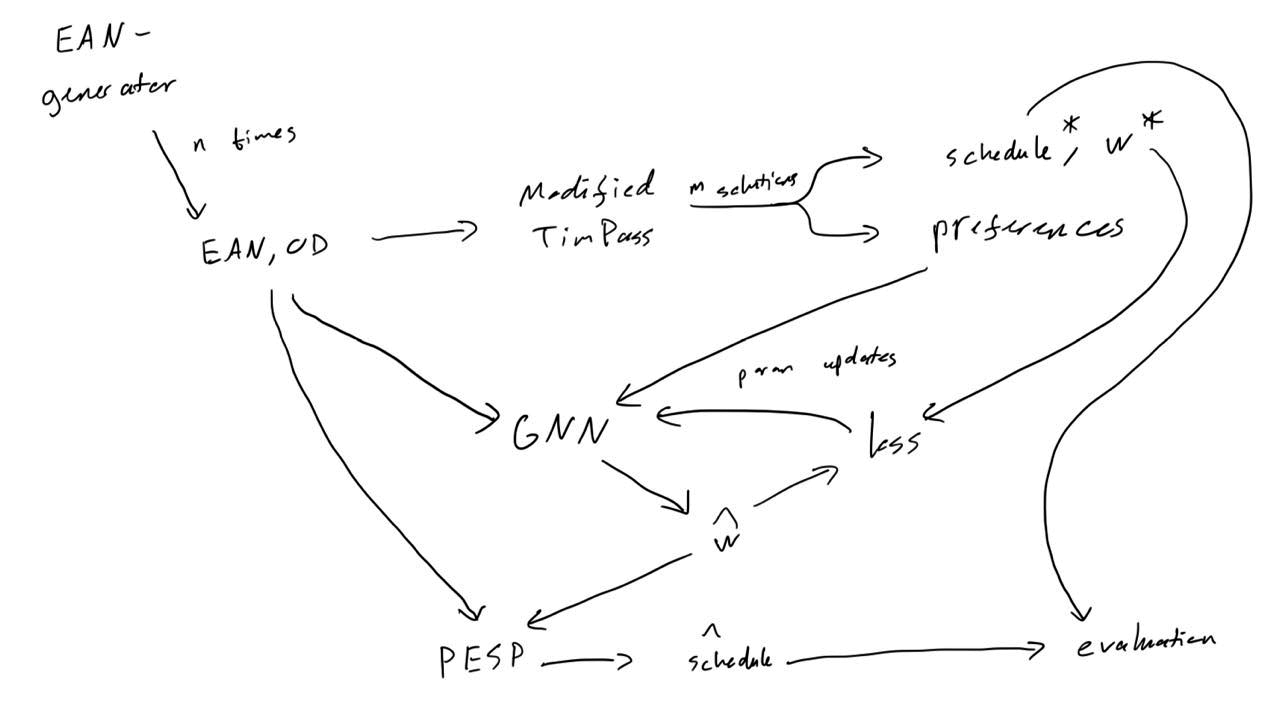
\includegraphics[width=\textwidth]{figures/process-flow.png}
    \caption{The overview of how the data is generated, model trained, and the heuristic evaluated.}
    \label{fig:process-flow}
\end{figure}
\subsection{Event activity network data}
\label{sec:ean-def}


% \begin{definition}[Public transport network]\label{def:ptn}
%     A public transport network (PTN) is a graph with a set of stops $V$ connected by a set of direct connections between the stops $E$. We consider the edges to be undirected.
% \end{definition}


% In \cref{def:ptn} we showed xyz.

% prujaa: ???


Before we can define event activity networks, we have to define a few other things.
\begin{definition}[Public Transport Network]\label{def:ptn}
    A \textit{public transport network} (PTN) is a simple undirected graph PTN = $(S, R)$ with a set of stops $S$ and a set of direct connections between the stops $R$. 
\end{definition}

A PTN describes the underlying transportation infrastructure of a public transport system. We consider the connections to be undirected. This simplifies the modeling, but one could also have a PTN with directed edges. The PTN could also be non-simple, but that notation would make a difference only if there were either capacity constraints per connection or if multiple modalities were used.

Stops and connections are not enough to model the public transport network. We will use an event activity network (EAN) for that.
\begin{definition}[Event Activity Network]\label{def:ean}
    The event activity network $EAN$ is a directed graph $\textit{EAN} = (E, A)$ with a set of events $E$ and a set of activities $A$ connecting the events.
\end{definition}
We will define the set of events $E$ and activities $A$ a bit later, as we need the notation of a line concept for that first.

\begin{definition}[Periodic scheduling] 
    A period $\period \in \N$ defines the time interval at which various events are repeated.
\end{definition}

We are interested in the periodic instead of the aperiodic scheduling problem. This period could be for example 60 minutes, one day, or something else. The appropriate period length depends on what kind of schedule we aim to optimise. %Note that in general, the period could be a positive real number, but we consider it to be an integer to follow the convention established in \cite{schiewe2020periodic}.

\begin{definition}[Line concept]
    A \textit{line} $l \subset R$ is a simple directed path in a PTN. A \textit{line concept} is a set of lines $L$ with associated frequencies $f_l \in \N$ for all $l \in L$. A frequency determines how often a line is served within the period $T$.
\end{definition}

% TODO: miten merkataan simple path tässä tapauksessa? Onko siis ordered setti / lista stoppeja?
%A \textit{line} $l \subset R$ is a simple directed path in a PTN. A \textit{line concept} is a set of lines $L$ with associated frequencies $f_l \in \N$ for all $l \in L$. A frequency determines how often a line is served within the period $T$. %We assume the lines to be bidirectional, meaning that the vehicles travel the line in both directions.

Here we assume the lines to be directed, meaning that vehicles travel the line only in one direction. Usually, in real-world lines, the vehicles travel in both directions, but this can also be modeled here by including the reverse direction as a separate line instance. %This notation of the line including the direction just makes the rest of the notation a bit simpler, while at the same time allowing more flexibility in what kinds of lines can be expressed.

From the line concept, we can define the set of events $E$ and activities $A$ used in the EAN.
% \begin{definition}[Event Activity Network]\label{def:ean}
%     The event activity network $EAN$ is a directed graph $\textit{EAN} = (E, A)$ with a set of events $E$ and a set of activities $A$ connecting the events.
% \end{definition}
For the events, we have the disjoint arrival and departure types: $E = \Earr \cup \Edep$. As the names suggest, the sets $\Earr$ and $\Edep$ contain the events describing vehicle arrivals and departures at the stops. To simplify the notation, we define the set of available repetition numbers as $R_l = \{1, \dots, f_l\}$. More formally, the sets are defined as follows:
\begin{align*}
    \Earr &= \{
        (\text{arr}, u, l, r) : l \in L, u \in l, r \in R_l
    \} \\
    \Edep &= \{
        (\text{dep}, u, l, r) : l \in L, u \in l, r \in R_l
    \}
\end{align*}
As seen in the definition, the events consist of the event type, the stop, the line, and the line repetition number which is used to differentiate between separate repetitions of the line in the periodic case.

For the activities, we also have multiple distinct types: drive, wait, change, and sync. Thus, we have that $A = A_\text{drive} \cup A_\text{wait} \cup A_\text{change} \cup \Async$. The formal definitions are as follows:
\begin{align*}
    A_\text{drive} =& \{(
        (\text{dep}, u, l, r),
        (\text{arr}, v, l, r)
    ): l \in L, (u, v) \in l, r \in R_l\}\\
    A_\text{wait} =& \{(
        (\text{arr}, u, l, r),
        (\text{dep}, u, l, r)
    ): l \in L, u \in l, r \in R_l\} \\
    A_\text{change} =& \{(
        (\text{arr}, u, l_1, r_1),
        (\text{dep}, u, l_2, r_2)
    ): \\&\quad (l_1, l_2) \in L^2, l_1 \neq l_2, u \in l_1 \cap l_2, r_1 \in R_{l_1}, r_2 \in R_{l_2}\} \\
    \Async =& \{(
       (t, u, l, r-1),
       (t, u, l, r)
    ): (t, u, l, r) \in E, r \geq 2 \}
\end{align*}

The drive activities correspond to the driving activity between stops. The activities connect the line's departure events to the corresponding arrival events. The wait activities correspond to the vehicle staying at the station, waiting for the passengers to board and disembark the vehicle. The wait activities connect arrival events to departure events. The drive and wait activities are demonstrated in \cref{fig:drive-wait-demo}. The change activities denote the line transfers that the passengers may take. The activities link the arrivals to departures within the same stop that do not belong to the same line. The idea of change activities and multiple lines at the same stop is shown in \cref{fig:change-demo}. The sync activities are slightly different from the other activities, as the passengers can not travel along those edges. For defining the optimization models, we note the set of activities usable for passenger routing as $\Ar = A \setminus \Async$. The purpose of sync activities is to define constraints on the timetable to have some predefined spacing among the repetitions of the lines. How sync activities are connected is shown in \cref{fig:sync-demo}. Defining the constraints on all sync activities is not mandatory. In that case, the sync activities without constraints are redundant.


\begin{figure}
    \centering
    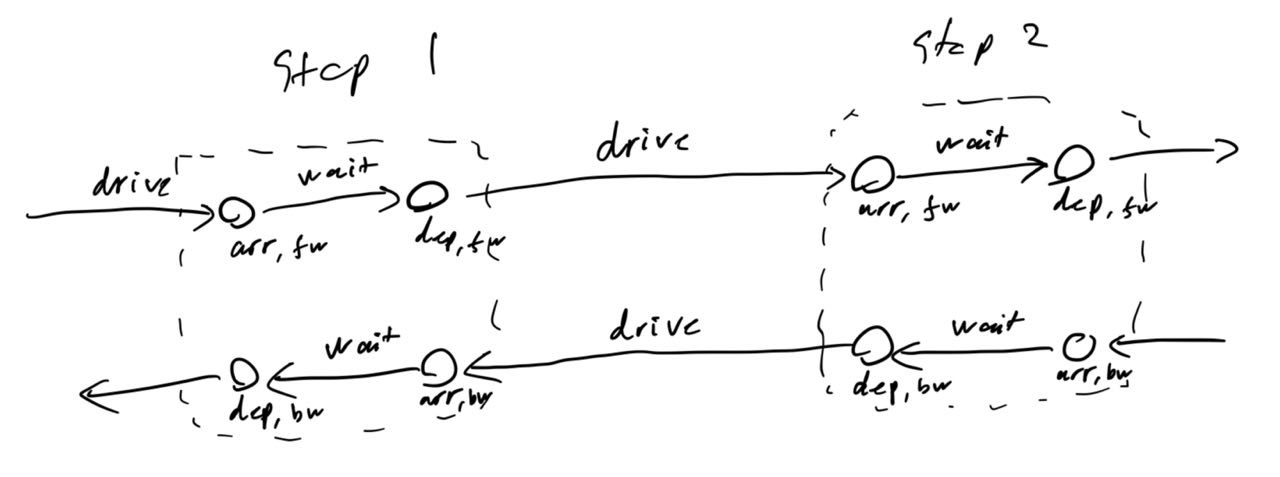
\includegraphics[width=1.0\textwidth]{figures/drive-wait-demo.jpg}
    \caption{Demonstration for arrival and departure events, drive and wait activities, and line directions.}
    \label{fig:drive-wait-demo}
\end{figure}

\begin{figure}
    \centering
    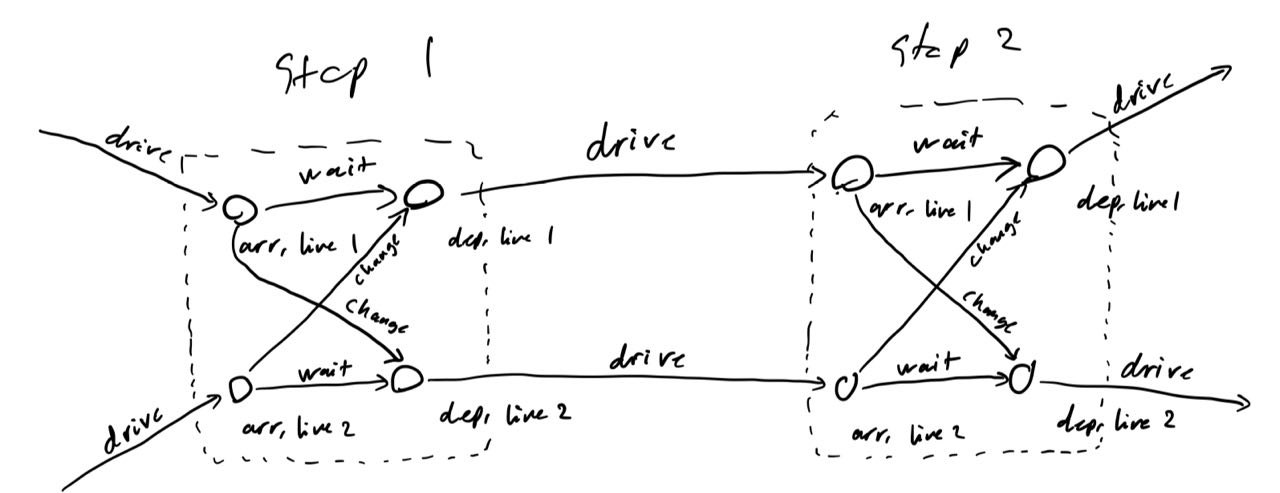
\includegraphics[width=1.0\textwidth]{figures/change-demo.jpg}
    \caption{Demonstration for multiple lines at a stop and change activities.}
    \label{fig:change-demo}
\end{figure}

\begin{figure}
    \centering
    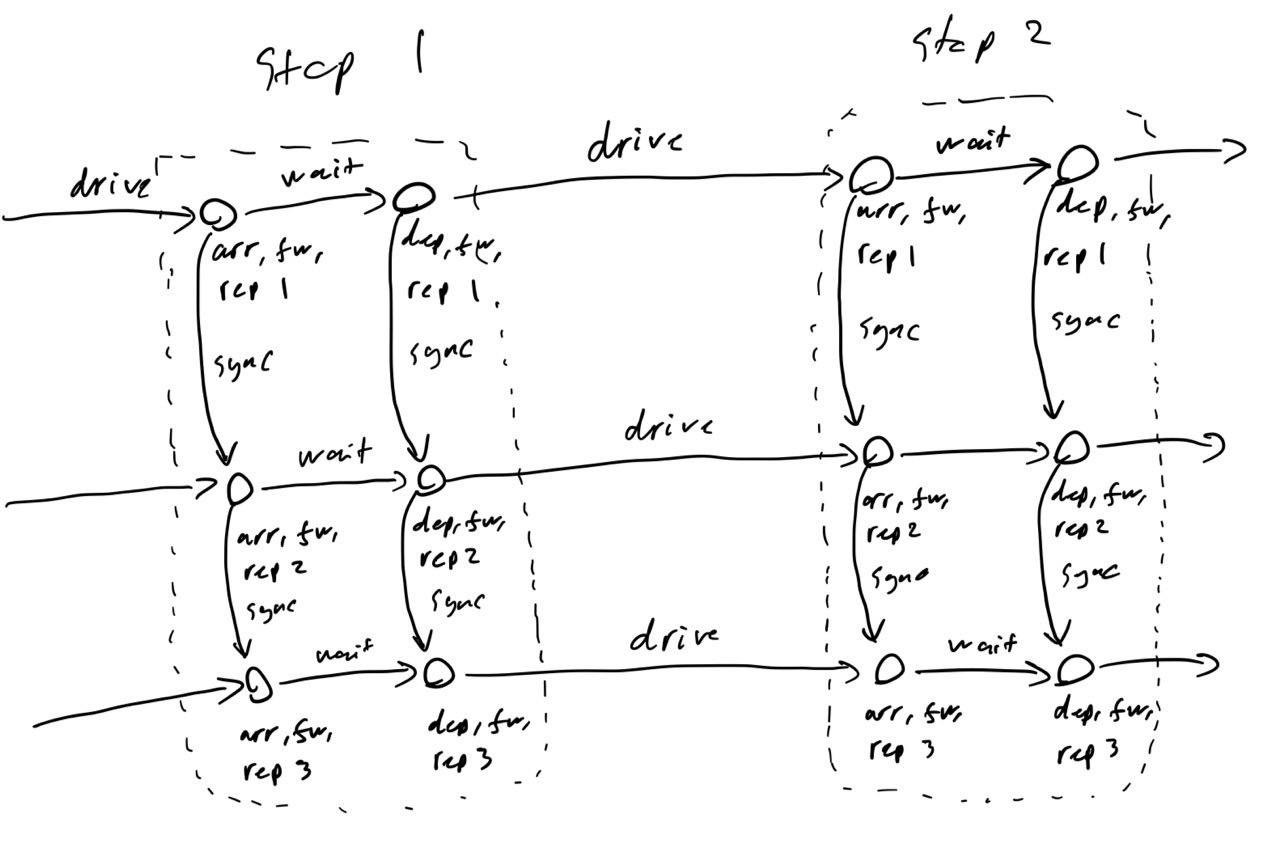
\includegraphics[width=1.0\textwidth]{figures/sync-demo.jpg}
    \caption{Demonstration for higher frequency lines and sync activities.}
    \label{fig:sync-demo}
\end{figure}

\subsection{Integer programming formulations}
\label{sec:ips}

Next we will define the integer programming formulations used. We will start with the periodic event scheduling problem (PESP) and it's cycle basis formulation. Then, we extend the PESP problem with passenger routing to obtain the time tabling and passenger routing (TimPass) problem.

\subsubsection{Periodic event scheduling problem}

The PESP problem in first presented in \cite{pesp-original-1989}. We will follow the formulation in \cite{schiewe2020periodic} with notation adapted to be in line with our definition of the EAN. In periodic scheduling, we have a periodic schedule $\pi$ defined for the events in the EAN. The event times are noted as $\pi_i \in \{0, \dots, T-1\}$ for all events $i \in E$. As we are working with a periodic schedule, all the event occurrence times must be lower than the period of the schedule $T$. %As noted previously, we could have a real-valued schedule instead of a discrete one, but once again we follow the previous formulation.

The activities in the EAN are used to define constraints on the upper and lower bounds for activity durations. For all activities $a \in A$, we have the lower bound $L_a \in \N$ and upper bound $U_a \in \N$. For the bounds, we of course must also have that $0 \leq L_a \leq U_a$. The activity duration for activity $a = (i, j)$ itself is calculated as $(\pi_j - \pi_i - L_a)\ \text{mod}\ T + L_a$. The lower bound term outside of the modulo ensures, that the lower bound is respected. The term inside the modulo is the "slack" time we have due to the schedule not aligning perfectly with the lower bound. As formulated, the duration is guaranteed to be greater or equal to the lower bound. For the given timetable $\pi$ to be feasible, for all activities $a \in A$ we must have that the upper bound holds: $(\pi_j - \pi_i - L_a)\ \text{mod}\ T + L_a\leq U_a$.

As the modulo operator does not fit well into linear programming as is, we replace the modulo with an integer multiple of the period $T$. The multiplier $z_a \in \Z$ becomes a decision variable. The lower bounds terms cancel out and the expression for the edge duration is now $\pi_j - \pi_i + z_aT$. As the multiplier $z_a$ can be chosen freely, this is equivalent to the formulation with the modulo.


In addition to the EAN, we need information on the passenger demand between the stops of the PTN. We note the number of passengers wanting to travel from stop $u$ to stop $v$ as $\od_{u, v} \in \N$. Not all stop pairs have demand: we express the set of stop pairs with non-zero demand as $\od = \{(u,v): (u, v) \in S \times S, \od_{u,v} > 0\}$.

For routing of the passengers, we assume a fixed routing that is given beforehand. When routing the passengers, each OD pair assumes some path from $u$ to $v$ through the EAN, and for the chosen path edges the weight $w_a$ is incremented by the number of passengers using that route. We will later return to routing in a subsequent section. For now, it's enough to recognize, that we have a weight $w_a \in \N$ for all routable activities $a \in \Ar$ of the EAN.

The total travel time given a timetable is expressed as $\sum_{a=(i,j) \in \Ar} w_a (\pi_j - \pi_i + z_aT) $. In PESP, we try to minimise this by searching for good timetables $\pi$. However, when routing the passengers given a timetable, the passengers may not always choose the fastest route, as inconveniences, e.g. transfers, affect the route decision. We model this by including a penalty $b_a > 0$, $a \in A$  that is considered when routing the passengers. In practice, we use shortest path routing but add the penalty to the transfer activity duration.

The total penalised travel time is $\sum_{a=(i,j) \in \Ar} w_a (\pi_j - \pi_i + z_aT + b_a)$. Note, that as $w_a$ and $b_a$ do not depend on $\pi$, we can substitute this as the PESP objective without affecting the optimal timetable. The new objective is equal to the total travel time plus a constant $\sum_{a \in \Ar}w_ab_a$. However, we prefer this objective formulation, as it will be directly comparable with the TimPass model objective defined in \cref{eq:timpass-obj}.

%Now we can express the PESP problem. Instead of minimizing the real total travel time $\sum_{a=(i,j) \in \Ar} w_a (\pi_j - \pi_i + z_aT)$, we minimize the total perceived travel time. In perceived travel time, we add the "perceived penalty" duration to the real duration. In principle, the penalty $b_a$ could be any real value, but in this case, we consider it to be a non-negative integer. This models the dissatisfaction of the people who have to change lines to get to their destination.

Note, that the objective only considers the routable activities, but the constraints take all activities into account.
\begin{align}
    \mathbf{(PESP)}\quad\min&\ \sum_{a \in \Ar} w_{a} (\pi_j-\pi_i+z_aT + b_a) \\
    \textrm{s.t.} \quad L_a &\leq \pi_j-\pi_i+z_aT  \leq U_a  &a &=(i,j)\in A \\
    \pi_i &\in \{0, \dots, T-1\} &i &\in E\\
    z_a &\in \Z &a &\in A
\end{align}

% From the OD demand, we use some routing scheme to obtain weights.  % TODO: more formally, good points in prev. literature.


The formulation for the PESP problem using the schedule $\pi$ is correct, but it's not the most efficient one available. As presented in \cite{cycle-basis-original-2001}, instead of explicitly defining the times for the events, we could instead define just the activity durations directly. We note the activity duration as $x_a \in \N$. Now the constraint on activity durations is much simpler: $L_a \leq x_a \leq U_a\ \forall a \in A$. This formulation also implicitly reduces the number of symmetrical solutions: when directly defining the event times by $\pi$ we would need to fix some event time explicitly to prevent symmetrical solutions from being considered.
% TODO: any research on why the cycle-basis is more efficient?

We still need to take the cycles and their feasibility in the EAN into account. In \cref{fig:cycle-example}, we have the activities a, b, c, d, e, and f. For the activity durations to be consistent, we must have that the difference of duration of the upper path $x_a + x_b + x_c$ and lower path $x_f + x_e + x_d$ must be an integer multiple of the period $T$. More formally, $x_a + x_b + x_c - x_d - x_e - x_f = zT$ for some $z\in \Z$. The difference can be a multiple of the period as we are dealing with a periodic timetable, otherwise the difference should be zero.

\begin{figure}
    \centering
    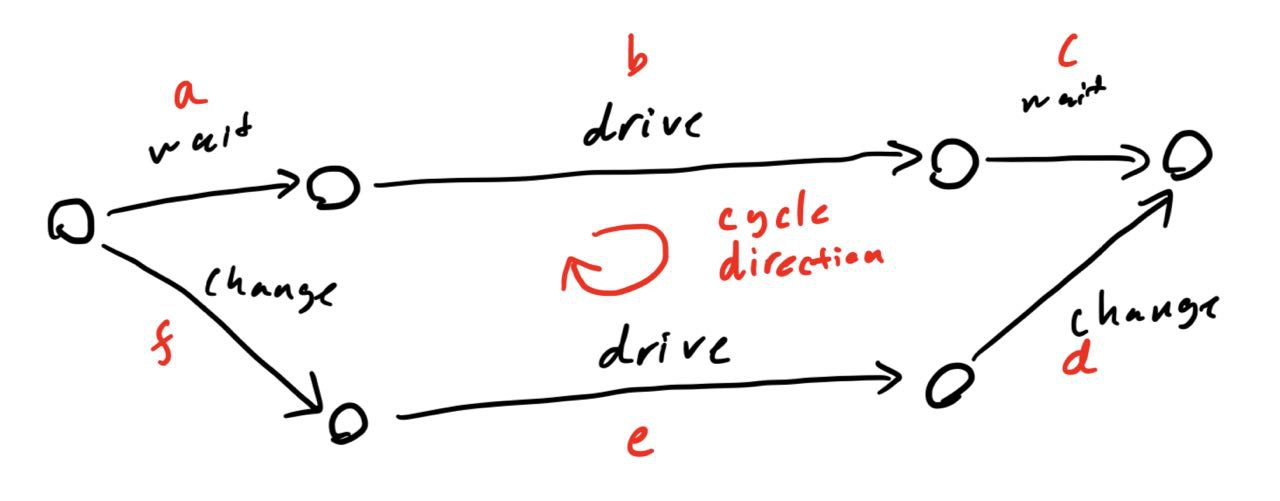
\includegraphics[width=\textwidth]{figures/cycle-basis-demo.jpg}
    \caption{Cycle consistency example.}
    \label{fig:cycle-example}
\end{figure}

% \begin{figure}
%     \centering
%     % \begin{tikzpicture}[
%     %     roundnode/.style={circle, draw=green!60, fill=green!5, very thick, minimum size=7mm},
%     %     squarednode/.style={rectangle, draw=red!60, fill=red!5, very thick, minimum size=5mm},
%     %     ]
%     %     %Nodes
%     %     \node[squarednode]      (maintopic)                              {2};
%     %     \node[roundnode]        (uppercircle)       [above=of maintopic] {1};
%     %     \node[squarednode]      (rightsquare)       [right=of maintopic] {3};
%     %     \node[roundnode]        (lowercircle)       [below=of maintopic] {4};
        
%     %     %Lines
%     %     \draw[->] (uppercircle.south) -- (maintopic.north);
%     %     \draw[->] (maintopic.east) -- (rightsquare.west);
%     %     \draw[->] (rightsquare.south) .. controls +(down:7mm) and +(right:7mm) .. (lowercircle.east);
        
%     % \end{tikzpicture}
%     \begin{tikzpicture}[
    round/.style={circle, draw=black, fill=white, very thick, minimum size=7mm},
    ]

    %Nodes
    \node[round] (s1-a1) at (0,0) {};
    \node[round] (s1-d1) at (2,0) {};
    \node[round] (s1-d2) at (4,0) {};
    \node[round] (s2-a1) at (0,-2) {};
    \node[round] (s2-a2) at (2,-2) {};
    \node[round] (s2-d1) at (4,-2) {};
    

    %Lines
    \draw[->] (s1-a1.east) -- (s1-d1.west);
    \draw[->] (s1-d1) -- (s2-a1);
    \draw[->] (s2-a1) -- (s2-d1);
    
    
\end{tikzpicture}

%     \caption{Cycle consistency example.}
%     \label{fig:cycle-example-tikz}
% \end{figure}

\begin{definition}{(Cycles in a directed graph)}
    A list of activities $(a_1, a_2, \dots, a_n)$ is a simple cycle if 
    adjacent activities share one event: $|a_i\cap a_{j}| = 1$ for all $i = {1, \dots, n}$ and $j = (i - 1 ) \mod n$, and the events of the activities are visited exactly once: $|\cup_{i=1,\dots, n}a_i| = n$. The cycle activities are divided into a set of positive edges $c^+$ and negative edges $c^-$. The positive edges are defined as $c^+ = \{a_i = (e_1, e_2) : e_1 \in a_j, j = (i - 1) \mod n\}$. Likewise, $c^- = \{a_i : a_i \notin c^+\}$.
    % - all adjacent activities share a node
    % - no duplicated verticies
\end{definition}

In the cycle basis formulation, we consider cycles regardless of the edge direction, but the cycle does have a direction. All the edges of a cycle $c$ belong either to the set of "positive edges" $c^+$ or the set of "negative edges" $c^-$, based on the direction of the edges along the cycle. In the example of \cref{fig:cycle-example}, we would have that $c^+ = \{a, b, c\}$ and $c^- = \{d, e, f\}$. In more general terms, for a cycle $c$ to be consistent, for some $z \in \Z$ we must have:
\begin{align}
    \sum_{a\in c^+}x_a - \sum_{a \in c^-}x_a = zT
\end{align}

An EAN may have many cycles, but luckily we do not have to check the condition for all of them. Following \cite{cycle-basis-original-2001}, we can construct a cycle basis for the EAN and checking the condition only for the basis is enough. In short, a cycle basis is a subset of the graph's cycles that can be used to construct every other cycle in the graph. We denote the cycle basis as $C$. As the cycle inconsistency can be a problem only with activities with constraints, we calculate the cycle basis for activities that can have constraints, i.e. the set $A$.

% TODO: proof / cite a source showing that cycle basis is enough to check. Maybe some words on how the cycle basis is constructed?


Now we may define the cycle basis formulation for the PESP problem. The formulation is quite similar to the original definition, but now the activity duration is expressed in a very concise way and we have the additional cycle consistency constraint:
\begin{align}
    \textbf{(PESP cycle basis)}\ \min &  \sum_{a \in \Ar} w_{a} (x_a + b_a) \\
    \textrm{s.t.} \quad  z_c T &= \sum_{a\in c^+} x_a - \sum_{a\in c^-} x_a &c &\in C \\
    L_a &\leq x_a  \leq U_a &a &\in A \\
    z_c &\in \Z &c& \in C \\
    x_a &\in \Z &a& \in A
\end{align}


\subsubsection{Timetabling and passenger routing problem}


In the TimPass problem presented in \cite{timpass-original-2014}, we are free to choose the route used for each OD pair in addition to the timetable as we minimise the total perceived travel time. In PESP, we have fixed passenger counts $w_a$ per activity. In TimPass, we optimise the passenger routing and consequently the weights $w_a$ at the same time as we optimise the timetable. This yields better solutions, as it takes passenger behaviour into account. In general, the passengers prefer to use routes with the shortest travel time to get to their destination.

%This means, that we can find better solutions that also model the passenger behaviour as a consequence of the timetable at the same time.



However, to represent the routes from stop $u$ to stop $v$ in an EAN, we would prefer to have a single predefined node representing the start of paths from stop $u$ and likewise a single node representing the end of the path at stop $v$. This is contrast to the path starting from or ending at some node in the set of events belonging to a stop. To achieve this, we introduce the auxiliary events $\Eaux$ and auxiliary activities $\Aaux$. 

\begin{definition}[Auxiliary events and activities]
    Each stop $u \in S$ of a PTN is associated with an auxiliary origin and destination event: \begin{align*}
        \Eaux = \{(t, u) : t \in \{\text{orig}, \text{dest}\}, u \in S\}
    \end{align*}
    Each auxiliary event is connected via auxiliary activities to the corresponding events in the EAN:
    \begin{align*}
        \Aaux = \bigcup_{i = (t, u, l, r) \in E}\{((\text{orig}, u), i), (i, (\text{dest}, u))\}
    \end{align*} 
\end{definition}
The auxiliary event and activity construction is demonstrated in \ref{fig:aux-events-demo}. Now, when considering a route from stop $u$ to $v$, we know that the path starts from $(\text{orig}, u)$ and ends at $(\text{dest}, v)$.

To denote the set of all routable activities, we note $\Arp = \Ar \cup \Aaux$. Similarly, to denote all events including the auxiliary events, we note $\Ep = E \cup \Eaux$. Auxiliary activities are not considered to be actual activities in the sense of not having a duration. As such, the auxiliary activities are not subject to duration constraints and are not part of the objective function.

% For the auxiliary events, we have one origin and destination event for each stop: $\Eaux = \{(t, u) : t \in \{\text{orig}, \text{dest}\}, u \in S\}$. For the auxiliary activities, we have an edge from all auxiliary origin events to the corresponding stop's events and an edge from all stop's events to the corresponding destination auxiliary event:
% \begin{align}
    %     \Aaux = \bigcup_{i = (t, u, l, r) \in E}\{((\text{orig}, u), i), (i, (\text{dest}, u))\}
%     % \Aaux = \{((\text{orig}, u), e): e = (t, u, l, r) \in E\} \cup 
%     % \{(e, (\text{dest}, u)): e = (t, u, l, r) \in E\}\\
% \end{align}


\begin{figure}[b]
    \centering
    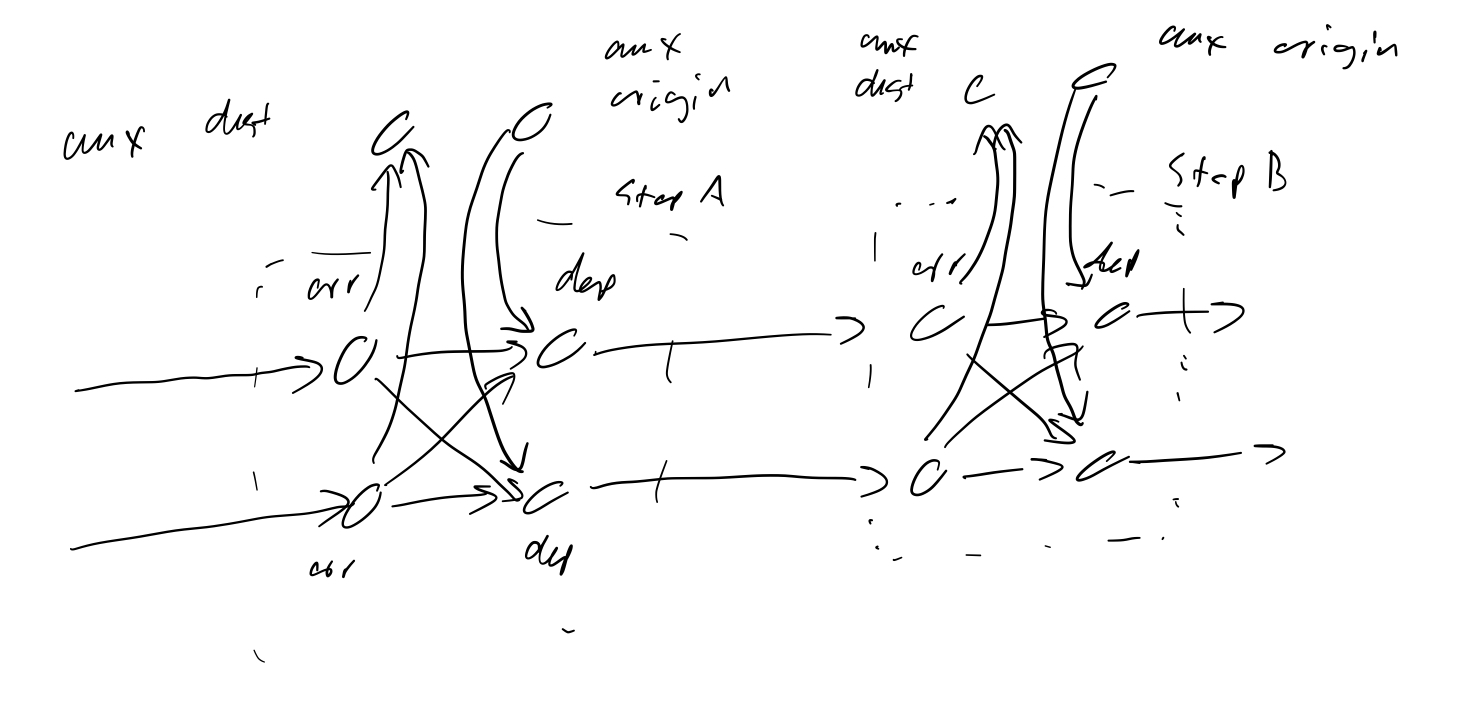
\includegraphics[width=0.8\textwidth]{figures/aux-events-demo.jpeg}
    \caption{Demonstration of how auxiliary events are connected to the rest of the EAN.}
    \label{fig:aux-events-demo}
\end{figure}

To note if the activity $a$ is part of the chosen path between stops $u$ and $v$, we have the flow variable $p_a^{uv} \in \{0, 1\}, (a, uv) \in \Arp \times \od$. This allows us to set up some constraints on what is considered a valid path. For a path from stop $u$ to stop $v$ to be valid, it must start at the event $(\text{orig}, u)$ and end at $(\text{dest}, v)$. Additionally, the path must be connected from the origin all the way to the destination, i.e., for all events that are not auxiliary events we must have an equal number of ingoing and outgoing activities that are used in the path. The activity is used to route from $u$ to $v$ if the corresponding flow variable is one: $p_a^{uv} = 1$.

We can formalise this by introducing a node-arc-incidence matrix $\incidence$ and an origin-destination vector $q^\mathit{uv} =(q_i^\mathit{uv})_{i\in \Ep}$. For a origin-destination pair $(u, v) \in \od$, the origin-destination vector elements are:
\begin{align}
    q^\mathit{uv}_i = \begin{cases}
        -1&\text{if}\ i=(\text{orig}, u)\\
        1&\text{if}\ i=(\text{dest}, v)\\
        0&\text{otherwise}
    \end{cases}
\end{align}

For the node-arc incidence matrix $\incidence=(m_{i, a})_{(i, a) \in \Ep \times \Arp}$, we have that the element is minus one if the activity leads away from the event, one if the activity leads to the event and zero otherwise. Formally:
\begin{align}
    m_{i, a} = \begin{cases}
        -1&\text{if}\ a = (i, j)\ \exists j \in \Ep\\
        1&\text{if}\  a = (j, i)\ \exists j \in \Ep\\
        0&\text{otherwise}
    \end{cases}
\end{align}

Armed with this notation, we can finally construct the constraint necessary for the set of active flow variables to constitute a valid path from stop $u$ to stop $v$:
\begin{align}
    \incidence (p_a^{uv})_{a \in \Arp} = q^\mathit{uv} \quad \forall uv \in \od
\end{align}
This constraint does not actually prevent the flow variables from creating a cycle, but as we are minimising the total perceived travel time, those cycles would be non-optimal and thus they will not occur in optimal solutions.

We can express the total perceived travel time as the sum of perceived travel times over all OD pairs. Thus, we are minimising the following expression:
\begin{align}
    \sum_{uv \in \od}\od_{uv} \sum_{a \in \Ar}p_a^{uv}(x_a + b_a)
\end{align}
However, we have a problem as we hope to get a linear integer programming problem. Now we have $p_a^{uv}x_a$, which is not linear as both terms are decision variables. Luckily, as the flow variable $p_a^{uv}$ can only be either 0 or 1, we can linearise this expression easily.

We create the linearization decision variable $\textit{lin}_a^{uv}$ for all $a \in \Ar$ and $uv \in \od$. We aim to always have $\textit{lin}_a^{uv} = p_a^{uv}(x_a + b_a)$ without explicitly stating this equality, as the right-hand side has the non-linear term. We achieve this by constructing suitable constraints for the linearization term.

Let $B$ be some large integer for which $B \geq x_a + b_a\ \forall a \in \Ar$. With this value, we can come up with the following set of constraints:
\begin{align}
    &\textit{lin}_a^{uv} \geq 0 \\
    &\textit{lin}_a^{uv} \leq p_a^{uv} B \\
    &\textit{lin}_a^{uv} \leq x_a + b_a \\
    &\textit{lin}_a^{uv} \geq x_a + b_a - (1 - p_a^{uv}) B
\end{align}
Now, if $p_a^{uv} = 0$, we must have that $\textit{lin}_a^{uv} = 0$. If $p_a^{uv} = 1$, then $\textit{lin}_a^{uv} = x_a + b_a$.

Now we can finally express the TimPass problem with the cycle basis formulation. We omit the linearization term and constraints for clarity, but in practice, the linearization must be done for commonly available solvers to function properly.
\begin{align}
    \textbf{(TimPass)}\ \min&\sum_{\mathit{uv} \in \textrm{OD}} \od_{\mathit{uv}} \sum_{a \in \Ar} p_{a}^{\mathit{uv}} (x_a + b_a) \label{eq:timpass-obj}\\
    % \textrm{min.} \quad  \sum_{\mathit{uv} \in \textrm{OD}} \od_{\mathit{uv}} \sum_{a \in A_\text{routable}} lin_a^{uv}) \\
    \textrm{s.t.} \quad  z_c T &= \sum_{a\in c^+} x_a - \sum_{a\in c^-} x_a &c& \in C \\
    L_a &\leq x_a \leq U_a &a& \in A \\
    \incidence (p_{a}^{\mathit{uv}})_{a\in \Arp} &= q^{\mathit{uv}} &\mathit{uv} &\in \textrm{OD}\\
    x_a &\in \Z &a& \in A \\
    z_c &\in \Z &c& \in C \\
    p_a^{\mathit{uv}} &\in \{0, 1\} &a& \in \Arp, \mathit{uv} \in \textrm{OD}
\end{align}

% \begin{itemize}
%     % \item Introduce auxiliary events used in the TimPass formulation.
%     % \item Introduce how the routing constraint matrix $A$ and vector $b$ are defined.
%     % \item Briefly describe how the linearization trick for the objective works.
%     % \item Describe how preprocessing works to reduce the number of routes we have to consider.
%     \item Describe how multiple solutions are obtained by turning the optimal objective into a constraint and generating a new objective with random weights on the routing variables. Maybe we can cite Helmi's work here?
% \end{itemize}

The given formulation for the TimPass problem works, but we are left with many flow variables. Luckily, there is a way to reduce the complexity by calculating which flows can never exist in the optimal solution. This method is first presented in \cite{schiewe2020periodic}. 


To formalise the preprocessing, we will need a notation for the shortest paths. In practice, the shortest paths will be calculated with Dijkstra's algorithm.
\begin{definition}[Shortest Path]
    Let $D$ be the vector of durations for activities so that $D_a \in \N$. We calculate the length of a path $P$ as $\len(P, D) = \sum_{a \in P} D_a$. We define the function $\shortestpath_{i,j}(D)$ to return a shortest path between the events $i$ and $j$, i.e. \begin{align}
        \min_P\  \len(P, D) = \len(\shortestpath_{i, j}(D), D)
    \end{align}
    Where $P$ is a valid path between events $i$ and $j$.
\end{definition}

% We define the function $\shortestpath_{u,v}(D)$ to be the function, that given the set of durations $D$ for the activities, calculates the shortest path between nodes $u$ and $v$ in the given EAN. This shortest path can be calculated with e.g. Dijkstra's algorithm. We can calculate the length of the path with the function $\mathit{len}(p, D)$, which calculates the length of the path $p$ with the durations $D$. We define $\mathit{len}(p, D) = \sum_{a \in p} D_a$.

The upper and lower bounds can be used as the duration in both $\len$ and $\shortestpath$. However, as in the TimPass problem we are dealing with perceived travel times, we should include the penalty term in the duration. Thus, let us define $L^b = \{L_a + b_a:a\in A\}$ and $U^b = \{U_a + b_a:a \in A\}$. Now we can use these to calculate which flow variables $p_a^{uv}$ can never be active in the optimal solution.

In \cref{alg:preprocessing} we present the algorithm for calculating which flow variables can be safely set to zero. We need to run the algorithm for each OD pair for which we want to reduce the number of flow variables. On a high level, the algorithm first calculates the longest possible route that can belong to an optimal solution. The length of that route under the upper bound edge durations is $\beta$. Then, for each activity, we check if the activity can belong to an optimal solution by checking if including the activity would increase the lowest possible perceived travel time for the path above $\beta$. In the end, we obtain a set of activities $\preprocessed_{uv}$, for which we can set the corresponding flow variable to zero. We handle the preprocessing by including the following constraint in the model:
%Let us note the set of preprocessed activities for the OD pair $uv \in \od$ as $P_{uv}$. This is the variable $P$ for running the algorithm for the given OD pair. 
%Then we can include the following constraint to handle the preprocessed flow variables:
\begin{align}
    p_a^{uv} = 0 \quad \forall uv \in \od, a \in \preprocessed_{uv}
\end{align}

% TODO: does this even make sense to represent this way? Definitions in a for loop may not be the most interesting thing.

\begin{algorithm}
    \caption{Flow variable preprocessing for OD pair $(u, v)$.}
    \label{alg:preprocessing}
    \begin{algorithmic}
        \State Auxiliary event $i = (\text{orig}, u)$
        \State Auxiliary event $j = (\text{dest}, v)$
        \State Initialise $\preprocessed_{uv} \gets \emptyset$
        \State Calculate $\beta := \mathit{len}(\shortestpath_{i, j}(U^b), U^b)$
        \Comment{Longest possible route length from $i$ to $j$.}
        \For{$k \in \Ep$}
            \State Calculate $\gamma_k := \mathit{len}(\shortestpath_{i,k}(L^b), L^b)$
            \Comment{Shortest possible path length from $i$ to $k$}
            \State Calculate $\delta_k := \mathit{len}(\shortestpath_{k,j}(L^b), L^b)$
            \Comment{Shortest possible path length from $k$ to $j$}
        \EndFor
        \For{$a = (i, j) \in \Arp$}
            \If{$\gamma_i + L_a^b + \delta_j > \beta$}
                \State $\preprocessed_{uv} \gets \preprocessed_{uv} \cup \{a\}$
                \Comment{The activity can never belong to the shortest path with any timetable, so we ignore it.}
            \EndIf
        \EndFor
    \end{algorithmic}
\end{algorithm}
    
\subsection{Shortest path routing heuristic}
\label{sec:sp-heur}

A simple baseline heuristic to the TimPass problem is to route the passengers according to the lower bound shortest paths and to then solve the timetable with PESP. Formally, we calculate the weights with \cref{alg:weights} by using the penalised lower bounds $L^b$ as the activity durations. As we don't have capacity constraints on the activities, we can route each OD pair independently of each other.

% TODO: citation to some relevant source

\begin{algorithm}
    \caption{Weight calculation from edge durations}
    \label{alg:weights}
    \begin{algorithmic}
        \Require{Activity durations $D$}
        \State $w_a = 0$ for all $a \in A$.
        \For{$(u, v) \in \od$}
            \State $i = (\mathrm{orig}, u)$
            \State $j = (\mathrm{dest}, v)$
            \For{$a \in \shortestpath_{i, j}(D)$}
                % \State $w_a \gets w_a + D_a$
                \State $w_a \gets w_a + \od_\mathit{u,v}$
            \EndFor
        \EndFor
    \end{algorithmic}
\end{algorithm}

We use the obtained weights in the PESP to obtain a timetable. The timetable evaluation is conducted in the same way as for the new proposed heuristic. The evaluation method is described in \cref{sec:heur-eval}. Note, that despite the weights used here representing real passengers, we should still do the rerouting as described in the evaluation method, as that can improve the objective. We want to ensure fair evaluation for both the baseline and the proposed heuristic.

% TODO: source / citation for why rerouting is necessary for fair evaluation

% \begin{itemize}
%     % \item Idea: use lower bounds + penalties as the edge duration, use Dijkstra's alg to calculate the shortest paths between each OD pair -> accumulate demand for OD pair to be a weight / demand for each activity along the shortest path.
%     \item Use obtained weights in PESP
%     \item Note about routing: we assume, that the passengers are happy to leave at any time during the period. We are minimizing just the time passengers spend going from origin stop to destination stop.
%     \item Note about capacity restrictions: as we don't have any, routing everyone through the same route is fine.
% \end{itemize}

\subsection{Graph Neural Networks}
\label{sec:gnns}

In general, neural networks are machine learning models with a large number of learnable parameters. The networks consist of multiple additions and multiplications in many layers. Even though the individual operations seem simple, surprisingly complex behaviour can emerge. Graph neural networks (GNNs) are a set of architectures that operate on graph data. To be specific, we focus here on message-passing architectures \cite{mpgnn-into-2017}, but other methods for processing graph data do exist.

In GNNs, the graph $G = (V, E)$ contains the node-level features $x_v, v\in V$ and edge-level features $e_{vw}, (vw) \in E$. We note the neighbourhood of node $v \in V$ as $N(v) = \{w : (v, w) \in E\}\subseteq V$. 
The GNN as in \cite{gnn-intro-2009} is viewed as a function $f:G \times V \to \R^m$ that maps the node $v \in V$ of a graph $G$ into $m$-dimensional Euclidian space. Essentially, this generates some $\R^m$ representations for the nodes that we can then use for other downstream tasks, e.g. regression or classification. In \cite{mpgnn-into-2017} the message-passing framework is introduced as a way to formalise the various variants of the graph neural networks.
In message-passing GNNs (MPGNNs), the neighbourhoods are used to pass messages between nodes that are used to update the states of the nodes. This differs from the other large class of GNNs that use the spectral representation of graphs \cite{gnn-review-2020}.

The algorithm contains multiple layers of message passing and processing, which ultimately yields the mapping or embedding of the nodes. We note the number of layers as $T$. For each layer $t$, we learn a message construction function $M_t$ and a state updating function $U_t$. The combination of the functions is used to construct the hidden states of the nodes $h_v^{t+1}$ for the next layer $t+1$.

The message construction function $M_t(h_v^t, h_w^t, e_{vw}),\ w \in N(v)$ maps the hidden states and the edge features of the neighbourhood of $v$ to messages. These messages can then be aggregated in some symmetric way, e.g. a sum in case of the messages belonging to some Euclidean space. The requirement for the aggregation to be symmetric is important: otherwise the hidden state update would depend on the order in which we process the edges, but this is not justified by the structure of the graph. The messages from the neighbourhood are aggregated to a single aggregated message $m_v^t$:
\begin{align}
    m_v^t = \sum_{w \in N(v)}M_t(h_v^t, h_w^t, e_{vw})
\end{align}

The state update function maps the current hidden state and the obtained aggregated message to a new hidden state: $h_v^{t+1} = U_t(h_v^t, m_v^t)$. This forms a layer together with the message generation and aggregation functions. The layers are repeated multiple times, each one with their own trainable parameters.

The obtained node embeddings $h_v^T$ of the last layer are used as inputs for the downstream tasks. For example, in the case of a regression problem, we can have a single-layer perceptron, mapping $h_v^T \mapsto \hat{y} \in \R$. Then, in a supervised setting, we can calculate the loss $\ell(y, \hat{y}) \in \R$ against the true label $y$ and use some optimization algorithm to update the model parameters to minimise the loss.

Typically, an optimization method for neural networks uses some variation of the stochastic gradient descent (SGD). In SGD, the gradient of the loss w.r.t. $\hat{y}$ is propagated back through the network to obtain the gradient with respect to the parameters. In standard SGD, the gradients multiplied by a suitable step size would be used as the parameter update. However, it has been noted that this method is susceptible to getting stuck on local minima. In this thesis, we will be using the Adam optimizer \cite{adam-2014}, which can be viewed as an extension of SGD with momentum and step size adaption.

One desirable quality of MPGNNs is that the same model can be used with networks of varying sizes. This does not limit us to always have the same number of nodes and edges in the problem.



\subsubsection{Positional encodings}

One limitation of the message-passing framework is, that if the initial node features are equal, some non-isomorphic network structures may not be detected \cite{repr-limit-2020}. This can be resolved by injecting some structural information to the features of the nodes. In this case, we will be using Laplacian eigenvector positional encodings (Laplacian PE) \cite{LaPE-first-introduction-2003} to allow the model to better differentiate many kinds of structures.

Let $A$ be the adjacency matrix of a graph. The elements of the Laplacian matrix $L$ are then
\begin{align}
    L_{ij} = \begin{cases}
        A_{ij},\ i \neq j\\
        \sum_{k \in V} A_{ik},\ i = j
    \end{cases}
\end{align}
The Laplacian eigenvectors $\mathbf{f_i}$ are the eigenvectors of the Laplacian matrix. For the positional encoding, we would take the eigenvectors with $m$ largest corresponding eigenvalues and inject the resulting vector values to the nodes.

The sign of the eigenvectors can be arbitrary. This is why we choose only top-$m$ vectors, as when training the model we need to pick a random combination of signs. The model can learn the invariance to the sings symmetries much easier, as we have a limited number of possible combinations.

A naive way of implementing the positional encoding would be to just use some random ordering of the nodes. This has the flaw that we would need to train the model using all possible orderings of the nodes to make the model learn to be invariant to the actual order, and just use it for positional information. As we typically choose $m \ll |V|$, using the Laplacian eigenvectors for positional encoding makes the model training much easier.

We use the Laplacian PE implementation from \cite{LaPE-implementation-2020}.


\subsubsection{Network architecture}

The typical MPGNNs are designed for homogenous graphs, meaning that the nodes and edges have the same semantic meaning. However, in this thesis, we need to include also non-homogenous information, as on top of the events and activities we have the OD demands. This pushes us to use more contemporary methods that allow us to model heterogeneous graphs. We chose to use the Heterogenous Graph Transformer (HGT) architecture \cite{hgt-2020}. The HGT architecture also includes methods for dealing with "web-scale networks" and temporal graphs, but we will omit those methods, as the networks we are dealing with are much smaller and do not vary over time.

In heterogenous graphs $G = (\mathcal{V}, \mathcal{E}, \mathcal{A}, \mathcal{R})$, the nodes $v \in \mathcal{V}$ and edges $e \in \mathcal{E}$ are associated to node types $\mathcal{A}$ and edge types $\mathcal{R}$ by mapping functions $\tau: \mathcal{V} \to \mathcal{A}, v \mapsto \tau(v)$ and $\phi: \mathcal{E} \to \mathcal{R}, e \mapsto \phi(e)$. This allows us to define the meta-relation $\langle \tau(u), \phi(e), \tau(v)\rangle$ of an edge $e=(u,v)$. This meta-relation is the tuple of the origin and destination node types and the edge relation. Using the meta-relation we can comprehensively state what kind of interaction an edge expresses. This will be used later when defining the message-passing methods of the network. Note, that a node-type pair may have multiple kinds of relations, this is why we need to also include the type of the edge to the meta-relation.

% TODO: definne hyperparameters: layer count, hidden dim size, attention head count

As in the MPGNN architecture, the HGT also consists of multiple layers that generate messages and aggregate them over the neighbourhood of a node $v$ to generate the updated hidden state $h_v^t$. However, in a heterogeneous setting, the feature distributions of the nodes of different types are also assumed to be different. This motivates the use of different message generation and update functions for different meta-relations and node types. The architecture also uses an attention mechanism to give more weight to messages coming from nodes that the model estimates to be important.

We define the set of all edges from node $u$ to $v$ as $E(u, v)$. Note, that as the node pair may have multiple relation types, $E(u,v)$ is a set with possibly multiple elements,

At a high level, the HGT layer's embedding update function $U_t$ is defined as
\begin{align}
    % h^{t+1}_v = \underset{s \in N(v)}{\agg}(\tilde{h}_v^t)\\
    h^{t+1}_v &= U_t(h_v^t, m_v^t) = \Alin_{\tau(v)}(\sigma(m_v^t))+h_v^t
%     \tilde{h}_v^{t+1} &= \mathit{Vec}(\sum_{(u, v) \in \mathit{NE}(v)}\att(u, e, v) \odot \msg(u, e, v))\\
%     \att(u, e, v) &\in \R^{\text{num-heads}} \\
%     \msg(u, e, v) &\in \R^{\text{num-heads} \times \text{hidden-ch / num-heads}}
    % \tilde{h}_v^{t+1} &= \mathbin{\|}_{i \in {1, \dots, n_{h}}}\sum_{(u, v) \in \mathit{NE}(v)} \mathit{Att}^i(u, e, v) \mathit{Msg}^i(u, e, v) \\
    % \mathit{Att^i}(u, e, v) &= \mathit{Softmax}(\mathit{ATT-head^i}(u, e, v))_i
\end{align}
First, the update functions applies a non-linear transformation $\sigma$ and then a node-type dependent linear mapping $\Alin$. The mapped value is then added to the residual connection $h_v^t$ to obtain the updated state. The non-linear transformation used is the Gaussian Error Linear Unit \cite{gelus}. All linear mappings $\operatorname{*-lin}$ are mappings of form $\operatorname{*-lin}(x) = Ax + b$, $x \in \R^m$ with learnable parameters $A \in \R^m$ and $b \in \R$.
% The incumbent update $\tilde{h_v^{t+1}}$ is 

The HGT architecture uses multi-head attention when aggregating the messages from various neighbors. Attention is a mechanism that estimates the importance of various messages. The attention values are used to multiply the messages, essentially resulting in a weighted sum aggregation. The multi-head part means, that instead of doing the step above only once, we have multiple attention heads doing the same message-generation and weighted sums in parallel. This allows the model to better pay attention to multiple important inputs.

We note the set of outbound edges from node $v$ and the corresponding neighbors as $NE(v) = \{(u, e) : u \in N(v), e \in E(u, v)\}$. To obtain the aggregated message, we concatenate the weighted sums obtained from the attention heads. The aggregated message $m_v^t$ is calculated as:
\begin{align*}
    m_v^t = \sum_{(u, e) \in \mathit{NE}(v)} \operatorname{\Big\Vert}_{i = 1}^{n_{\mathit{heads}}} \underset{i, u, e, v}{\operatorname{SoftMax}}(\operatorname{Att-head}^i(u, e, v))\operatorname{MSG-head}^i(u, e, v)
\end{align*}  % NOTES: operaatioiden järjestys vähän hassu, mut oikein. NE määritelty näin, koska voi olla useampia edgejä nodejen välillä.

The message heads are defined as:
\begin{align*}
    \operatorname{MSG-head}^i(u, e, v) = \operatorname{M-Linear}^i_{\tau(u)}(h^{t}_u)W^{\text{msg}}_{\phi(e)}
\end{align*}
The message head value is calculated by first calculating a source node type-dependent linear mapping. This is then projected with an edge-type dependent matrix to form the message head.

The attention head yields scalar values that are then normalised with the SoftMax function over the neighbourhood of the node. The attention head is defined as:
\begin{align*}
    \operatorname{Att-head}^i(u, e, v) = \operatorname{K-linear}^i_{\tau(u)}(h^t_u)W^\text{att}_{\phi(e)}\operatorname{Q-linear}^i_{\tau(v)}(h^t_v)\frac{\mu_{u, e, v}}{\sqrt{d}}
\end{align*}
The attention head first maps the hidden states to a key and a query vector. Typically in attention calculation, we would then directly take the dot product of the vectors. However, this would not take the relation type into consideration. For this reason, we introduce a relation-dependant projection before the dot product. Finally, we scale the result based on a learnable scalar and the number of hidden dimensions $d$.


\subsection{Heuristic evaluation method}
\label{sec:heur-eval}


The GNN heuristic yields us weights for the activities in the EAN and with those weights we solve the schedule with PESP. However, we cannot directly calculate the TimPass objective value from the weights and the schedule, as the weights can be arbitrarily scaled so it does not represent the total number of passengers per activity. We will solve this by calculating the objective minimising properly scaled weights based on the obtained schedule. Luckily, this is easy to do, as the shortest path routing based on the obtained activity durations minimises the objective for the given schedule.

We will now show that the shortest path routing minimises the objective for a fixed schedule. Let $P(u, v)$ be a path between stops $u$ and $v$. The TimPass objective can formulated equivalently in terms of routes or paths instead of flow variables:
\begin{align}
    &\min_{P}\sum_{uv \in \od} \od_{uv} \sum_{a \in P(u, v)} x_a \\
    =&\min_{P}\sum_{uv \in \od} \od_{uv} \len(P(u, v), x)
\end{align}

Remember that we don't have capacity constraints for the activities. This means, that the paths are independent of each other. This means, that we can simply minimise each term of the sum independently. By the definition of the shortest path route $SP_{u, v}(x)$, the shortest path routing minimises this objective.

\begin{align}
    =&\sum_{uv \in \od} \od_{uv} \min_{P(u,v)}\len(P(u, v), x) \\
    =&\sum_{uv \in \od} \od_{uv} \len(\shortestpath_{(\mathrm{orig}, u),(\mathrm{dest}, v)}(x), x) \label{eq:eval-obj}
\end{align}

We calculate the objective value for the heuristic from \cref{eq:eval-obj} by setting $x$ to be the activity durations solved from the PESP. This value can be compared with both the shortest path heuristic and the TimPass solution's upper and lower bounds to determine how well the heuristic is doing.


% \begin{itemize}
%     \item For heuristics that assign weights to activities, that are then used to solve PESP
%     \item Process in short: solve pesp, use obtained time table to generate shortest path routing, calculate the real objective value from shortest paths and obtained event durations.
%     \item Reasoning for doing all this: the weights obtained from the GNN may be scaled arbitrarily (just a prediction, not necessarily unbiased / ) -> we must rescale the weights so that the weights represent 
% \end{itemize}

\clearpage
\section{Experiment setup}
\label{sec:experiments}
\subsection{Data generation}
\label{sec:data-gen}

To train the neural network, we generated a large number of EANs and ODs for which we can solve the TimPass problem to optimality in reasonable time. The problem typically has multiple solutions, but for reasons explained in \cref{sec:solution-preference-reasoning} we need to control which of the optimal solutions we obtain. All problems use the same PTN with varying lines, duration bounds, frequencies, demands, and penalties. We use a period $T$ of 60 minutes. The PTN is drawn in \cref{fig:base-ptn}.

Next we define the notation used for the uniform distribution in the algorithms. We use sampling of distributions to generate variations in the training data.
\begin{notation}[Uniform distributions]
    By $\mathcal{U}\{x, y\}$ we denote the discrete uniform distribution between $x \in \Z$ and $y\in \Z$, including endpoints. The continuous counterpart $\mathcal{U}[x, y]$ is the continuous uniform distribution between $x \in \R$ and $y \in \R$, excluding $y$. Note that the bracket type differentiates the continuous distribution from the discrete one.
\end{notation}


\begin{figure}
    \centering
    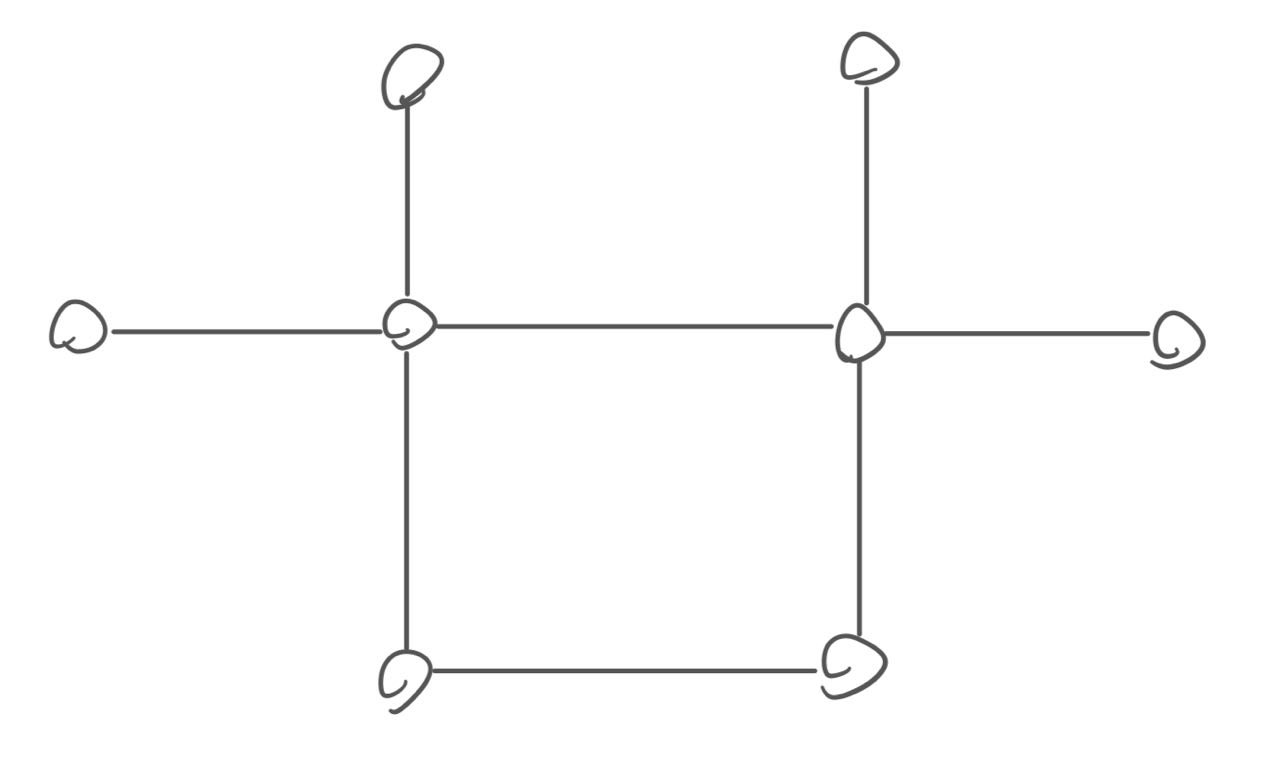
\includegraphics[width=0.8\textwidth]{figures/base-ptn.jpg}
    \caption{The base PTN on which we generate data.}
    \label{fig:base-ptn}
\end{figure}


First, we list all available lines as the set $\mathcal{L}$ with at least three stops and filter the reversed line versions out. To keep the line plan realistic, we later add the reverse line directions back to the plan. Then, we sample the line plan size $|L| \sim \unif{2, 4}$. Knowing the size, we sampled the lines belonging to the plan uniformly without replacement from the set of lines: $L \subset \mathcal{L}$. As we want to emulate real EANs, we check whether the resulting EAN would be connected if the reverse directions for the lines were also included. If this is not the case, we sample the line concept $L$ again.



After the set of lines is determined, we sample the line frequencies $f_l$ with the discrete probability mass function $p(f_l) = \sqrt[|L| - 1]{f_l / 4} - \sqrt[|L| - 1]{(f_l - 1) / 4}$. The probability mass function is visualised in \cref{fig:generation-rl-mass}. The function is designed to give a larger weight for the low line frequencies in case we have only a few lines in total. This regulates the variations in solving times for the generated problems. %In practice, the samples are generated from a uniform distribution: $f_l = \lfloor x ^{|L| - 1} / 4 \rfloor + 1, x \sim \unifcont{0, 1}$.  % skip, may be be confusing even though the methods are equivalent

\begin{figure}
    \centering
    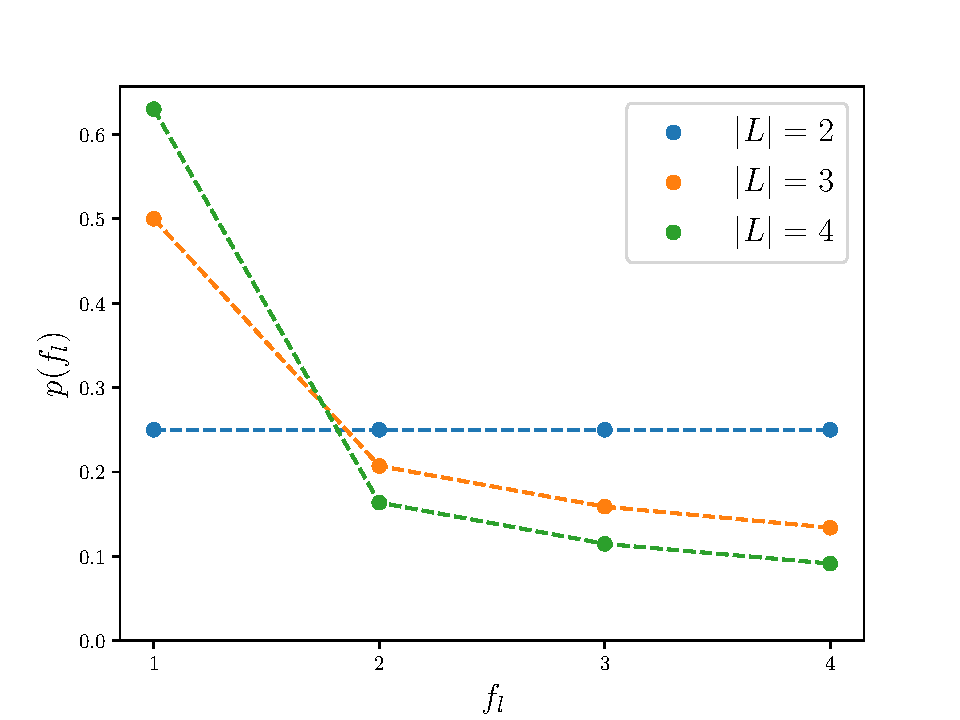
\includegraphics[width=0.8\textwidth]{figures/generation-rl-sample-density.pdf}
    \caption{Probability mass functions for the sampling distribution of $f_l$ with various sizes $|L|$.}
    \label{fig:generation-rl-mass}
\end{figure}


As we want the passengers to be able to travel everywhere in the resulting EAN, we also include the lines in the reverse direction. We define the reverse line $l_r$ of a line $l$ as $l_r = \{(j, i):(i, j) \in l\}$. For the EAN, we use the extended line set $L^r = L \cup \{l_r : l \in L \}$. We also set the frequency to the reverse direction to be the same as to the forward direction: $f_{l_r} = f_l$.

From the set of lines and frequencies, we can derive the events and activities of the EAN. We create all events and activities as defined in \cref{sec:ean-def}. For all activities, we also define the upper and lower bounds for the duration. We sample the bounds using \cref{alg:drive-sampling}. The algorithm first iterates through lines and relevant stop pairs. After sampling the bounds, the bounds are then set for all relevant activities.


\begin{algorithm}

\caption{Algorithm for sampling the drive activity duration bounds}
\label{alg:drive-sampling}
\begin{algorithmic}
    \For{$l \in L$}
        \For{$(u, v) \in l$}
            \State Sample $\lambda \sim \unif{1, 15}$ \Comment{The lower bound}
            \State Sample $\omega \sim \unif{0, 5}$ \Comment{Difference between upper and lower bound}
            \For{$r \in R_l$}
                \State $a_1 = ((\text{dep}, u, l, r), (\text{arr}, v, l, r))$ \Comment{Drive activity of $l$}
                \State $a_2 = ((\text{dep}, v, l_r, r), (\text{arr}, u, l_r, r))$ \Comment{Drive activity of $l_r$}
                \State $L_{a_1}, L_{a_2} = \lambda$
                \State $U_{a_1}, U_{a_2} = \lambda + \omega$
            \EndFor
        \EndFor
    \EndFor
\end{algorithmic}

\end{algorithm}

The bounds for wait activities are sampled with the same idea of not having the bounds change between line directions or repetitions. This time we loop over the stops and skip the iteration if the stop is the start or end of the given line. The method is described in \cref{alg:wait-sampling}

\begin{algorithm}

    \caption{Algorithm for sampling the wait activity duration bounds}
    \label{alg:wait-sampling}
    \begin{algorithmic}
        \For{$l \in L$}
            \For{$s \in l$}
                \If{$s$ is the start or end of $l$}
                    \State \textbf{Continue}
                \EndIf
                \State Sample $\lambda \sim \unif{1, 3}$ \Comment{The lower bound}
                \State Sample $\omega \sim \unif{0, 2}$ \Comment{Difference between upper and lower bound}
                \For{$r \in R_l$}
                    \State $a_1 = ((\text{arr}, u, l, r), (\text{dep}, u, l, r))$ \Comment{Wait activity of $l$}
                    \State $a_2 = ((\text{arr}, u, l_r, r), (\text{dep}, u, l_r, r))$ \Comment{Wait activity of $l_r$}
                    \State $L_{a_1}, L_{a_2} = \lambda$
                    \State $U_{a_1}, U_{a_2} = \lambda + \omega$
                \EndFor
            \EndFor
        \EndFor
    \end{algorithmic}
    
\end{algorithm}

For the change activities, the sampling process is a bit different. First, we sample the lower bound $\lambda_u \sim \unif{1, 5}$ for all $ u \in S$. Then, $L_a = \lambda_u,\ U_a = \lambda_u + T - 1$ for all activities $a = [(\text{arr}, u, l_1, r_1), (\text{dep}, u, l_2, r_2)] \in A_\text{change}$. In this case, the difference between the upper and lower bound is always $T-1$. This ensures, that the change is always feasible. We have the same bounds for all transfers that happen at the same stop.

By the definition used here, we could have different penalties for all the change activities, and nothing limits us to having penalties only for those activities either. However, to keep things simple and aligned with other datasets, we just sample $\rho \sim \unif{1, 5}$ and set $b_a = \rho$ for all $a \in A_\text{change}$ and $b_a = 0$ otherwise.

For sync activities, we don't sample the bounds. Instead, we simply set
\begin{align}
    L_a, U_a = T / f_l\quad  \forall a = ((t, u, l, r_1), (t, u, l, r_1)) \in \Async
\end{align}
Note, that $L_a, U_a \in \N$ as we chose $T$ and $f_l$ sampling to enforce this. This is necessary, as the TimPass model formulation is defined in terms of integers.

Finally, we must come up with an OD matrix for the problem instance. Only the stops that belong to a line are present in the EAN. As the lines are randomly chosen, the set of stops is also random. The shares of varying node set sizes in the dataset are presented in \cref{fig:data-node-count-shares}. 
%If we were to consider the demand for all stop pairs, we could end up with a difficult problem to solve, as we could have many OD-pairs for which we need to solve the best route.
To both keep the number of OD pairs feasible and to introduce variations in the data, we limit the number of OD pairs considered. When $|S| \geq 7$, the problem has at least $7 \cdot 6=42$ possible pairs. Instead of using them all, we take a random subset of the possible OD pairs. 
We sample $|\od| \sim \unif{30, 40}$ and then take the random subset $\od \subset S^2$. If we did not sample $|\od|$, we just use all possible OD-pairs. For all OD-pairs we sample the demand as $\od_{uv} \sim \unif{1, 20}$ for all $uv \in \od$.

\begin{figure}
    \centering
    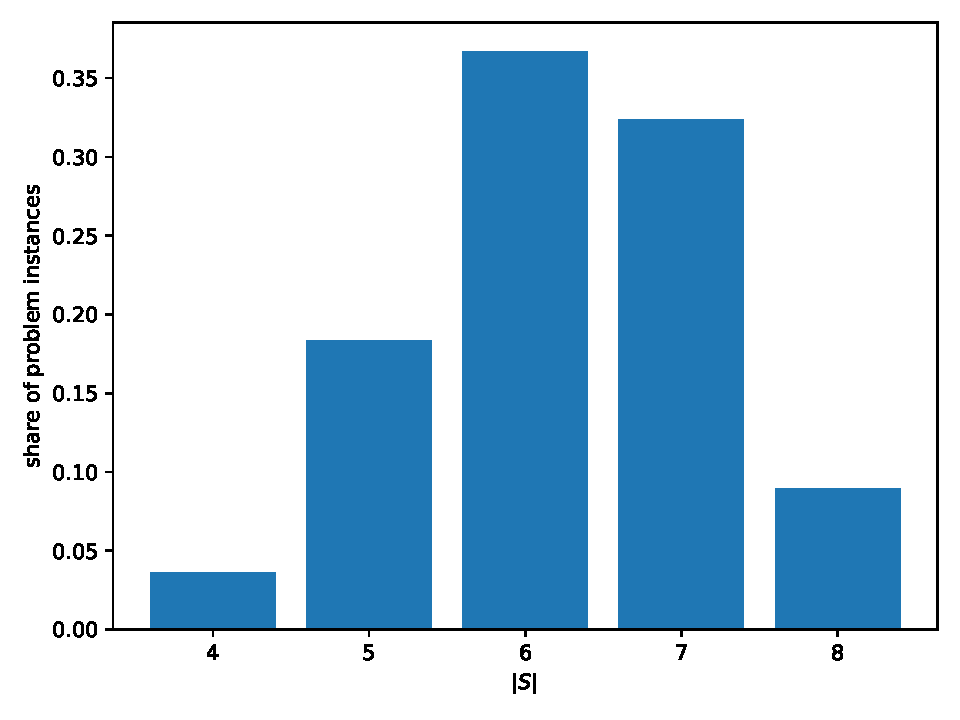
\includegraphics[width=0.75\textwidth]{figures/data_node_count_shares.pdf}
    \caption{Shares of node set sizes in the generated dataset.}
    \label{fig:data-node-count-shares}
\end{figure}

Now we can define the TimPass problem and attempt to solve it. We try to solve the obtained problem with Gurobi with a time limit of 20 seconds. If the optimal solution is not obtained within this limit, we deem the problem difficult to solve and try sampling the problem again. This happened in approximately $48\%$ of the sampled problem variations.

As stated previously, we need to be able to control which of the multiple solutions we actually get. This is done by first solving the problem as usual. We denote the calculated optimal objective value $V^*$. To obtain other solutions, we add a new constraint and change the objective function. The new constraint is that the objective must be equal to $V^*$:
\begin{align}
    \sum_{\mathit{uv} \in \textrm{OD}} \od_{\mathit{uv}} \sum_{a \in \Ar} p_{a}^{\mathit{uv}} (x_a + b_a)  = V^*
\end{align}
The idea for using the previous objective value as a constraint comes from \cite{helmi}.

For the new objective, we change it to be  the weighted sum of the flow variables. The weights are sampled randomly between zero and one:
\begin{align}
    \min\ \sum_{uv \in \od}\sum_{a\in \Ar}w_a^{uv}p_{a}^{\mathit{uv}} (x_a + b_a),\quad w_a^{uv} \sim \unifcont{0, 1}
\end{align}
Assuming that we can't sample the same weight for multiple flow variables, this ensures that the modified problem has only one optimal solution.

With the problem given above, we attempt to generate 10 solutions for each problem instance. We only keep the unique solutions. Then we write the solutions to disk to be used later for the neural network training and evaluation.

% TODO: comment on the number of solutions found???



% For the lines with a frequency greater than one, we generate sync activities between all events in sequential line repetitions. By setting the sync upper and lower bounds to be equal to the period divided by the line frequency, we ensure even spacing of the departures.


\subsection{Data representation as a heterogenous graph}
\label{sec:data-repr-graph}

% The simplified overview of the node types and their relations is expressed in \cref{fig:hetero-relations}. We use 
On top of the EAN data, we have the OD data we need to include as input to the GNN. We will use a heterogenous graph for this, as it allows us to include multiple kinds of nodes and relations in a graph. The simplified overview of the node types and their relations is expressed in \cref{fig:hetero-relations}.

The set of node types is $\mathcal{A} = \{\text{event}, \text{stop}, \text{line}\}$. As the line and stop ids are essentially meaningless on their own, we chose to represent the identity of a line and a stop as a separate node in the graph. This allows us to meaningfully represent which events belong to which stop and line without needing to e.g. permute the ids when training the model. The node type defines what kinds of features the node has. The line and stop type nodes do not have any features. The event-type nodes have one-hot encoded the event type, either arrival or departure.

The set of edge types is $\mathcal{R} = \{\text{activity}, \text{demand}, \text{belongs}\}$. The activity-type nodes have the activity type one-hot encoded. The activity duration lower bound $L_a$, upper bound $U_a$, and penalty $b_a$ are included as a share of the period $T$. The normalised shortest path routing weight is also included. In the preprocessing step we deduced that some of the flow variables must be zero. We chose to not encode this information as is, but as an aggregate of the share of flow variables that were preprocessed. We controlled for the optimal solution we obtained from the TimPass model with the preference variables.
%The preferences are also included in the features, as otherwise we could not determine which solution the GNN should aim for. 
To keep the regression target disambiguous, the preferences are also included in the features.
The demand edges store the number of customers wanting to travel between the stops. The value is normalised to have a maximum value of one across all edges. The belongs edge type does not contain any features.

Unfortunately, the implementation of HGT we are using does not use edge features directly. Instead, we will encode the edge features by connecting the line graph representation of the edges to the rest of the graph. A similar trick is used in \cite{line-graph-trick}. The method is visualised in \cref{fig:line-graph}. We applied the line-graph conversion one edge type at a time for the activity and demand edge types.

\begin{figure}
    \centering
    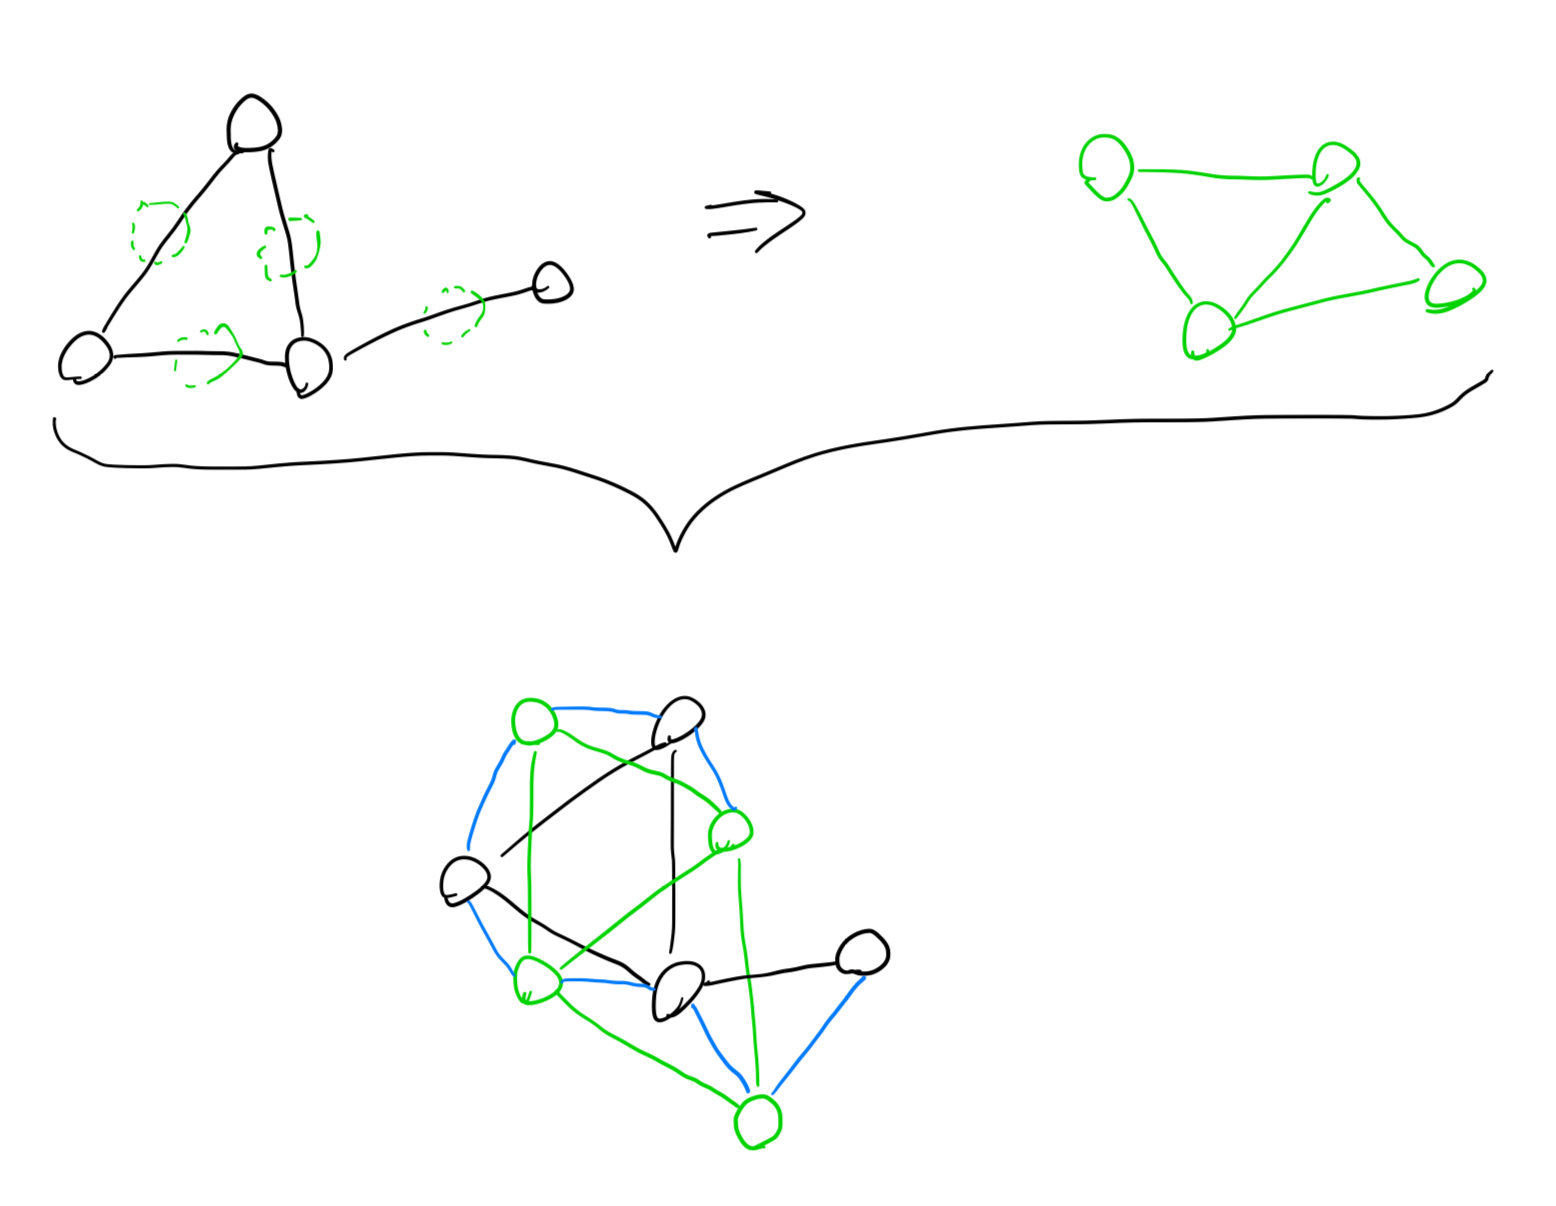
\includegraphics[width=\textwidth]{figures/line-graphs.jpeg}
    \caption{Demonstration of how the line graph trick is used to include edge features in the graph. The original graph with edge features is top left. The line graph of the edges on top right turns edges into nodes and connects the new nodes that were previously connected to a same node. The graphs are then joined by connecting the edge nodes to corresponding original nodes. The method is described in detail in \cref{alg:line-graph}.}
    \label{fig:line-graph}
\end{figure}


\begin{algorithm}

    \caption{Line graph extension}
    \label{alg:line-graph}
    \begin{algorithmic}
        \Require{Graph $G=(V,E)$}
        \State $E_{\text{line}} = \{(e, f) : (e, f) \in E^2, e\cap f \neq \emptyset\}$
        \Comment{The edge pairs that share an endpoint}
        \State $L(G) = (E, E_{\text{line}})$ \Comment{The line graph}
        \State $V_\text{joined} = V \cup E$
        \State $E_\text{joined} = E \cup E_\text{line} \cup \{(v, (v, n)) : v \in V, n \in N(v)\}$
        \State Joined graph $J = (V_\text{joined}, E_\text{joined})$
    \end{algorithmic}
    
\end{algorithm}
 

\begin{figure}
    \centering
    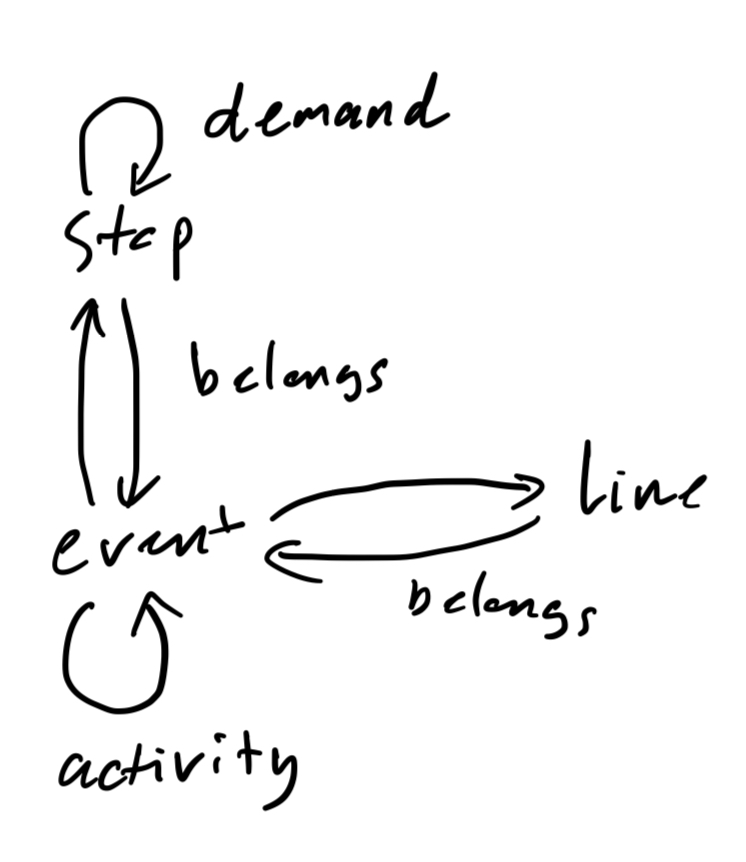
\includegraphics[width=0.3\textwidth]{figures/hetero-graph-relations.jpg}
    \caption{The node and relation types of the heterogenous representation.}
    \label{fig:hetero-relations}
\end{figure}
% \begin{itemize}
    % \item Describe how heterogenous graphs are represented in torch\_geometric -> some data conversions are needed
    % \item Edge features not included in the architecture -> we turn edges with features to nodes, connecting them with special edges to the original edge endpoints
    % \item Remove stop and line ids from features, describe how stops and lines are represented as only the identity of the id is important, not the ordering of the ids.
    % \item Additional feature: shortest path weights
    % \item Type one-hot encodings
    % \item Normalizations for values, easier for neural networks to learn this way
    % \item OD demand representation
    % \item Included metapaths, as otherwise edge feature nodes could suffer from the lack of connections. (part of the line graph trick)
% \end{itemize}


\subsection{Training}
\label{sec:training}

The HGT architecture and the training process are parametrized by hyperparameters. The hyperparameters for the HGT architecture are the number of hidden layers, the dimension of the hidden layers, and the number of attention heads used. The training process is 

\draft{   
    Hyperparams:
    - batch size (Mostly memory limit, also affects step )
    - number of layers
    - number of attention heads
    - number of hidden channels
    - learning rate
    Parallel training: multiple training agents, fetch testable parameters from the coordinating server
    Server assigns parameters based on strategy.
    Strategies:
    - grid (discrete "design space"?? check wording here), easily unnecessarily many combinations to test
    - random (works also with continuous variables), not too bad, but we can do better
    - bayesian (models expected value and expected variation, pick new samples from design space based on ?)
}
    
\draft{
    \begin{itemize}
        \item Describe hyperparameters and hyperparameter optimization with Bayesian search
        \item Trained on triton with xyz hardware
        \item Results in \cref{app:hyperparams}
    \end{itemize}
}
\clearpage
\section{Results}
\label{sec:results}
\subsection{Heuristic performance}
\label{sec:heur-perf}

\begin{figure}
    \begin{subfigure}{0.5\textwidth}
        \centering
        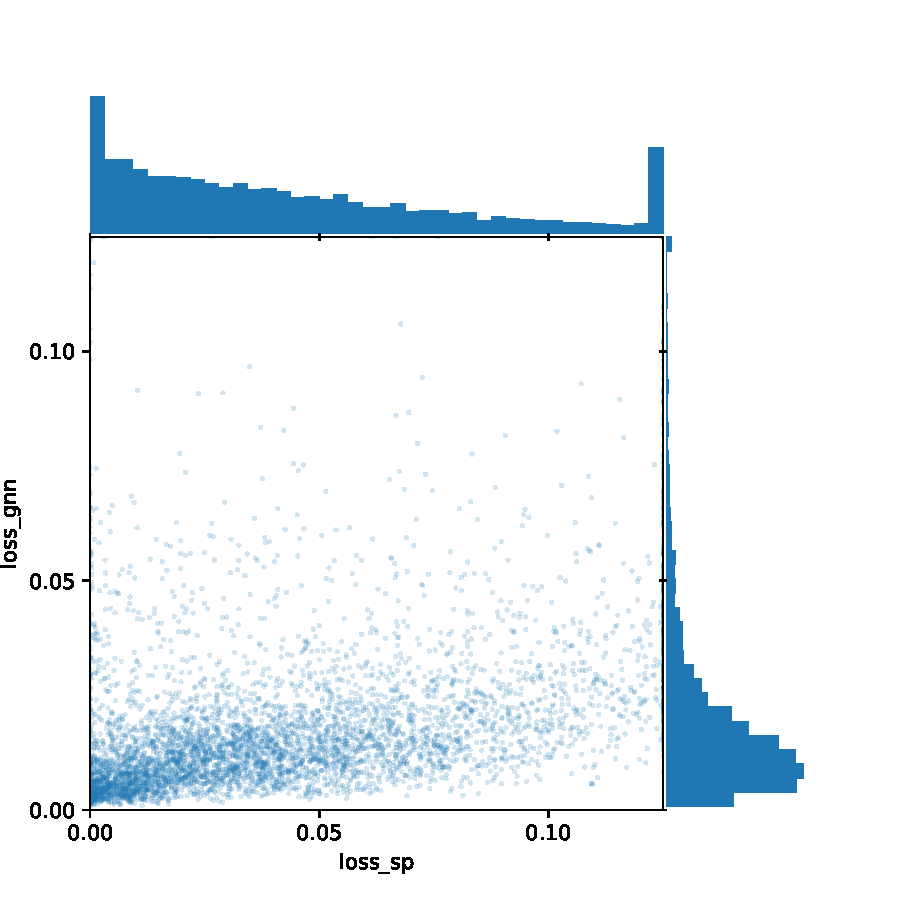
\includegraphics[width=\linewidth]{figures/loss-loss.pdf}
        \caption{Shortest path heuristic loss vs GNN loss.}
        \label{fig:results-ll}
    \end{subfigure}
    \begin{subfigure}{0.5\textwidth}
        \centering
        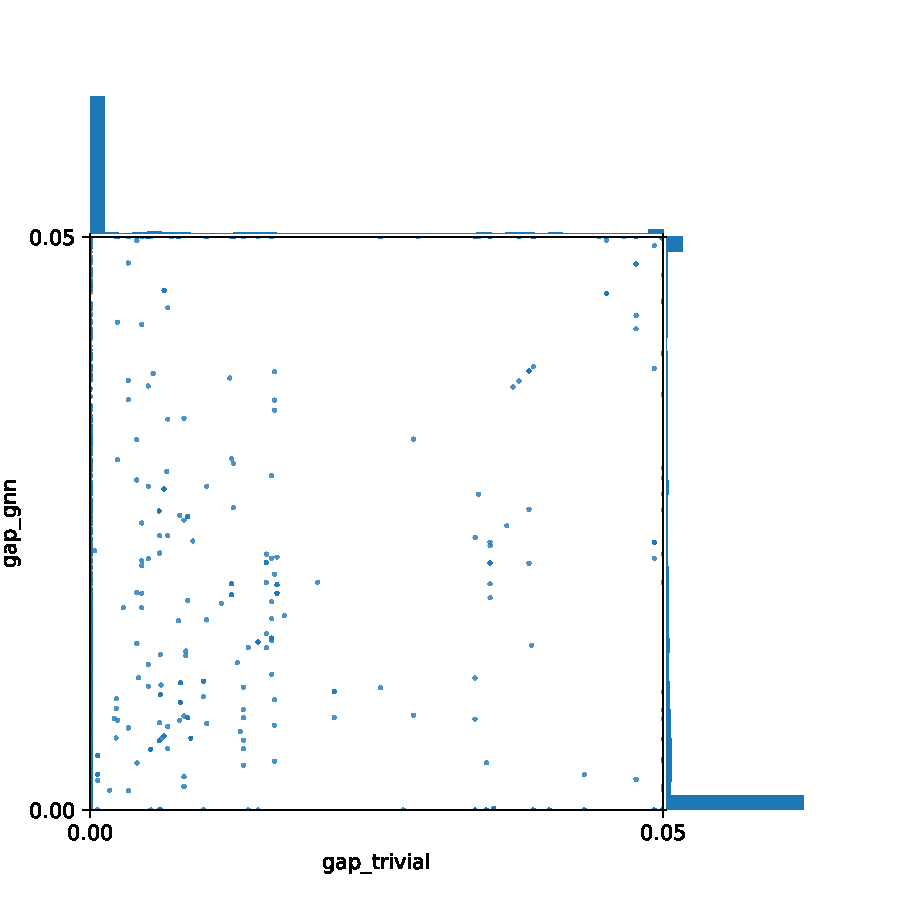
\includegraphics[width=\linewidth]{figures/gap-gap.pdf}
        \caption{Shortest path heuristic gap vs GNN gap.}
        \label{fig:results-gg}
    \end{subfigure}
    \caption{Join distributions for the shortest path heuristic and GNN performance metrics. Marginal distributions as histograms along the edges. The views are clipped slightly and the clipped values are collected in the last bins of the histograms.}
    \label{fig:results-ll-gg}
\end{figure}

We calculated the performance metrics on a test dataset with over 5000 samples. This dataset was not used in the training of the GNN heuristic.

For each problem instance, we calculated the GNN heuristic loss (as MSE against the optimal activity weights) and optimality gap as described in \cref{sec:heur-eval}. We also calculated the metrics for the shortest path heuristic weights. The heuristic is called the "trivial heuristic" in the figures. First, in \cref{fig:results-ll-gg} we compare the joint distributions of the losses and optimality gaps of the heuristic against each other.

For the calculated losses in \cref{fig:results-ll} we can clearly see, that the GNN heuristic typically achieves lower losses than the trivial heuristic. This indicates that the trained network did at least partially work as intended, as the heuristic was trained to minimise the loss. The loss is smaller for the GNN in 79\% of the problem instances.

However, observing the results in \cref{fig:results-gg} is more difficult. For the trivial heuristic, the gap is zero in 91\% of the cases and for the GNN heuristic in 61\%. Notably, the trivial heuristic finds the optimal solution more often than the GNN heuristic despite having larger losses. More on that in \cref{sec:loss-gap-relation}. However, we will now restrict our comparison to only cases where the trivial heuristic optimality gap is nonzero. We justify this condition by stating that the optimality of the trivial heuristic is easy to verify beforehand. As we are interested in improving the found solutions, we limit our focus only to cases where we know beforehand that improvements are possible. We use the name trivial problem for the problems where the shortest path heuristic achieves zero optimality gap.

In \cref{fig:results-gg-excl-trivial} we represent the optimality gap joint distribution without the trivial problems. Note, how the histograms are no longer concentrated around zero. With this filtering, the GNN heuristic achieves a better gap in 41\% of the problems. Likewise, the trivial heuristic has a better gap for 47\% of the problems. When the solutions differ, the difference is often quite large: if GNN gap is smaller, on average it is only about 31\% of the trivial heuristic gap. This means, that the proposed heuristic can find solutions that are vastly better than the baseline shortest path heuristic. However, this is not consistent.


\begin{figure}
    \centering
    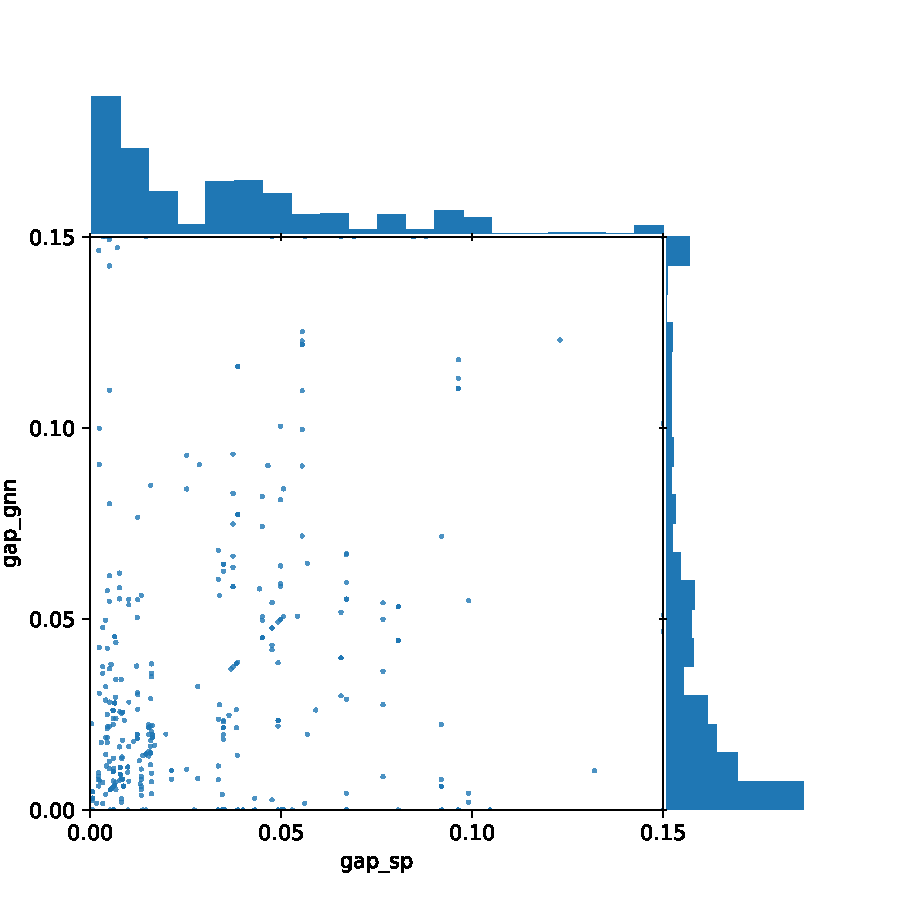
\includegraphics[width=0.75\linewidth]{figures/gap-gap-excl-trivials.pdf}
    \caption{Optimality gap joint distribution for trivial and GNN heuristics. Excluding trivial problems.}
    \label{fig:results-gg-excl-trivial}
\end{figure}

In \cref{tab:results} we present the calculated heuristic performance metrics in tabular form. 

We also evaluated the GNN and SP heuristics on selected TimPassLib instances. The benchmark instances are much larger and more diverse than the training problems. This allows us to probe the generalization ability and scalability of our heuristic approach. We compare the GNN heuristic results against the SP heuristic and the best published lower and upper bounds. The visualised results are represented in \cref{fig:eval-timpasslib}. As observed from the figure, the GNN heuristic yields much greater optimality gaps than the SP heuristic, regardless of the instance size. This hints, that the new method does not generalise well, as is a common limitation of many other ML approaches in combinatorial optimization (\cite{cappart2023combinatorial}).


The PESP time limit was set to 6 hours for the evaluation. The evaluation was performed on a machine with CPU 8 cores and 8 GB of memory. The problem instance sizes can be found in \cite{schiewe2023introducing}.
% TODO: aikaraja 6h, testataan generalization & scalability, kerro instanssien koosta jotain (näin monta eventtiä, aktiviteettia & od-paria)
\begin{figure}
    \centering
    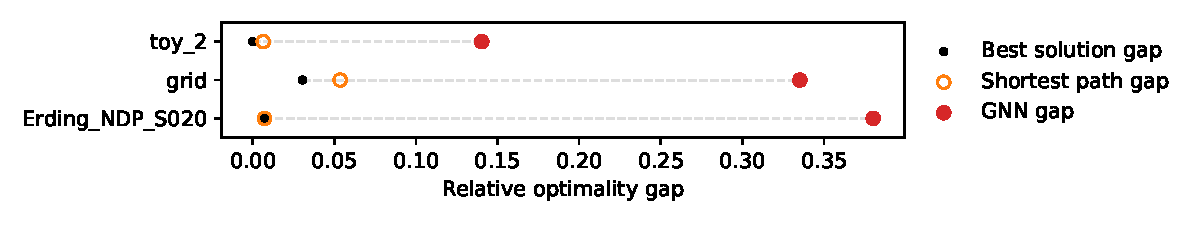
\includegraphics[width=\linewidth]{figures/eval-timpasslib.pdf}
    \caption{Optimality gaps with respect to the best bound published for the TimPassLib instance.} 
    \label{fig:eval-timpasslib}
\end{figure}

\begin{table}[]
    \centering
    \caption{Heuristic performance metrics both before and after filtering for trivial problem instances.}
    \label{tab:results}
    \footnotesize
    \begin{tabular}{l|ll|ll}
                                     & All problems  &                   & Non-trivial problems &                   \\
    Metric                           & GNN heuristic & Trivial heuristic & GNN heuristic        & Trivial heuristic \\ \hline
    Loss mean                        & \textbf{0.018526} & 0.045599          & \textbf{0.016793}    & 0.032772          \\
    Loss median                      & \textbf{0.013557} & 0.034702          & \textbf{0.013480}    & 0.022635          \\
    Gap mean                         & 0.011484          & \textbf{0.002880} & 0.036789             & \textbf{0.034759} \\
    Gap median                       & \textbf{0.000000} & \textbf{0.000000} & \textbf{0.019865}    & 0.025327          \\
    Loss smaller share               & \textbf{0.7851}   & 0.2149            & \textbf{0.7210}      & 0.2790            \\
    Gap smaller share                & 0.0349            & \textbf{0.3532}   & 0.4066               & \textbf{0.4657}   \\
    \makecell{Average relative\\gap improvement} &               &                   & 0.31                 &                  
    \end{tabular}
    \end{table}


\subsection{Relation of loss and heuristic optimality gap}
\label{sec:loss-gap-relation}

The chosen GNN heuristic training has the inbuilt assumption, that achieving good predictions for the optimal weights $w$ leads to low optimality gaps. However, after observing the achieved losses and optimality gaps for both the GNN and the trivial heuristic, this does not seem to be so straightforward.

In \cref{fig:gap-loss} we observe the loss vs optimality gap plots for both heuristics. If the assumption was correct, we would observe some kind of positive correlation between the metrics. However, the metrics are virtually independent of each other. Only when we focus on very small losses as in \cref{fig:gap-loss-gnn-zoomed} we see any dependence. For very small losses the optimality gaps tend to also be very small.


\begin{figure}
    \begin{subfigure}{0.5\textwidth}
        \centering
        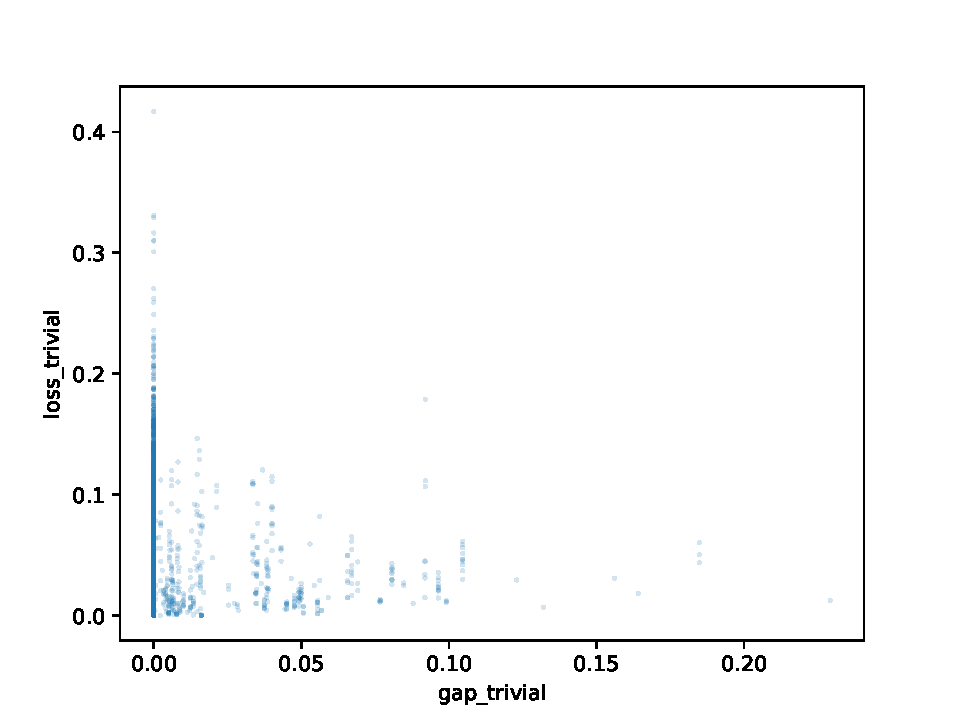
\includegraphics[width=\linewidth]{figures/gap-loss-trivial.pdf}
        \caption{Gap vs loss trivial heuristic}
        \label{fig:gap-loss-trivial}
    \end{subfigure}
    \begin{subfigure}{0.5\textwidth}
        \centering
        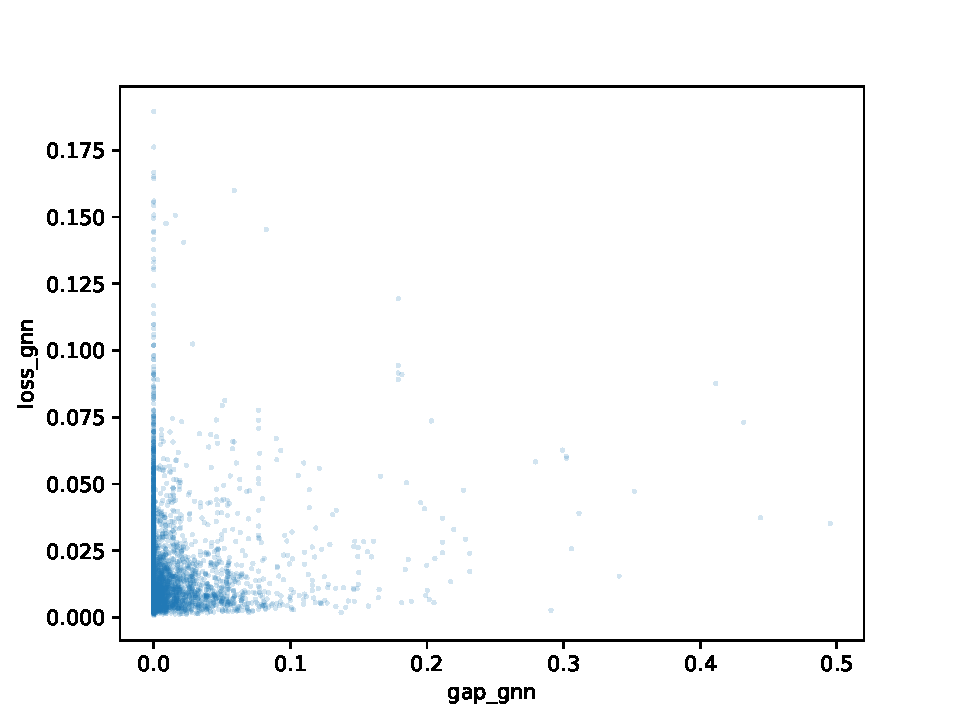
\includegraphics[width=\linewidth]{figures/gap-loss-gnn.pdf}
        \caption{Gap vs loss GNN heuristic}
        \label{fig:gap-loss-gnn}
    \end{subfigure}
    \caption{Relationship between the heuristic loss and the achieved optimality gap.}
    \label{fig:gap-loss}
\end{figure}

\begin{figure}
    \centering
    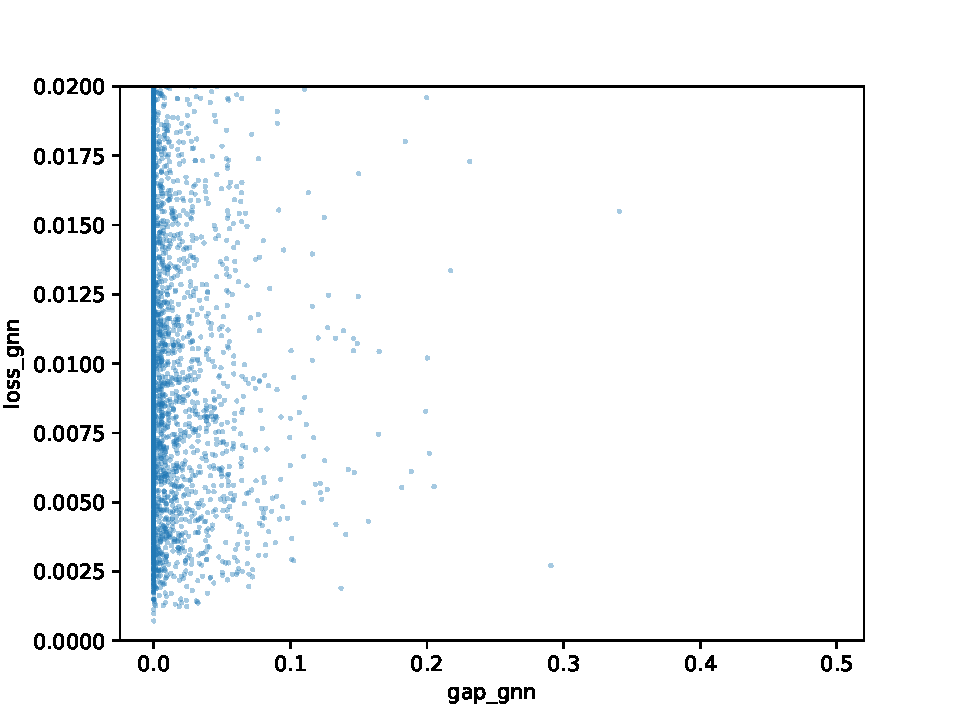
\includegraphics[width=0.8\linewidth]{figures/gap-loss-gnn-zoomed.pdf}
    \caption{Zoomed view to \cref{fig:gap-loss-gnn}. We observe, that for very low loss values the gap tends to also be zero.}
    \label{fig:gap-loss-gnn-zoomed}

\end{figure}

% \begin{itemize}
%     \item GNN heuristic has an inbuilt assumption that the optimality gap gets smaller as loss decreases
%     \item True when loss is very small, otherwise correlation is low
%     \item Plot of gap vs loss with both GNN and shortest path routing, points colored by heuristic
% \end{itemize}


\subsection{Theoretical loss lower bound without preference of solutions}
\label{sec:solution-preference-reasoning}

We will next investigate what would be the theoretically lowest obtainable loss if we did not include the preference information for the flow variables. As observed, for a given problem instance, we may have multiple optimal solutions to the TimPass problem. We assume that the optimal solution which we obtain is uniformly random between all optimal solutions if we do not control for this with the preference mechanism.

The neural network is trained to minimise the expected average squared error of the weight predictions. The loss for an individual problem is defined as $\ell(\hat{w}, w) = 1 / |A| \sum_{a \in A}(\hat{w}_a-w_a)^2$. If we don't consider preference information, then $w$ can be viewed as a random variable. In this case, the optimal predictor would predict $\hat{w}_a^* = \mathbb{E}[w_a]$. By substituting this back to the loss formula, we get that the lowest obtainable expected loss is the mean population variance of the weights, with the population here being the set of optimal solutions for one problem instance and the average being taken over all problem instances.

We can estimate this lowest obtainable loss by calculating the sample variances for the weights. With this method, we get that $\mathbb{E}[\ell(\hat{w}^*, w)] \approx 0.0091$. As this is lower than the best loss achieved with the preferences, we can deduce that the lack of preference information would not have limited the performance of the model significantly.

% \label{sec:solution-preference-reasoning}
% \begin{itemize}
%     \item Multiple solutions to TimPass exist, we pick the "right" one essentially at random
%     \item We are using mse loss -> the loss would be minimized when we predict the expected value of the optimal solution
%     \item Multiple solutions -> we are actually not predicting an optimal solution, but something else
%     \item Empirically, the lower bound for the loss would be the variance of the obtained weights
%     \item Got an estimate of 0.00199 -> we couldn't get a loss lower than that with this dataset without the preference order.
% \end{itemize}


\clearpage
\section{Discussion}
\label{sec:discussion}

As an overview of the obtained results, the GNN heuristic does not bring a consistent improvement against the SP heuristic. On non-trivial problems sampled from the same distribution as the training data, the new method may improve the results, but whether improvements are possible can not be known beforehand.

The instances in TimPassLib represent a different data distribution than the training data. By testing the GNN heuristic against the benchmark instances, we found that the GNN heuristic does not generalise well to distributions outside of the training data. One of the reasons we chose the GNN architecture for our heuristic was the technical feasibility of using the same network for problem instances of different sizes. As the capability to generalise was very weak, we did not manage to observe if the problem instance size plays a role in performance. The possible performance degradation due to scaling the instances was masked by the large optimality gaps due to generalisation issues.

The question remains if predicting the weights is a good idea in the first place. As we compared the optimality gaps against the $l^2$ loss on the weight prediction in \cref{sec:loss-gap-relation}, we did not observe any strong correlation between the values. This indicates, that training the model to predict the weight does not necessarily result in a lower gap against the reference solution. Additionally, as the allowed predictions were continuous, sometimes the low but non-zero weight values caused the subsequent PESP solving to be considerably slower than solving the PESP with the SP weights. % Pointti: vaikee ennustaa just nollaa

To get around these issues, we came up with two ideas for further research into the topic of using a NN heuristics for the routing part of the TimPass problem. First, instead of training the model to predict the weights, we could instead try to predict the routes. This would make sure, that the resulting weights are consistent with the passenger demands, allowing us to skip the SP rerouting in the evaluation phase. The second idea is to try to minimise the TimPass objective value itself by means of reinforcement learning. As improvements in the regression task do not directly translate to better objective values, we could try to to minimise the objective instead. However, RL training is much more difficult to get right than the simple supervised regression task.

Another point of discussion is the suitability of the HGT architecture for this problem. The family of convolutional graph networks are well-suited for tasks with local dependencies. This is also reflected in the typical benchmarks, e.g. (\# TODO: paper-author, joku muu kans). However, the task of routing the passengers optimally depends on global interactions: a small difference in the network, e.g. a high lower bound for an edge, may have large consequences far away, as now it's optimal to route the passengers with a completely different path to their destination.

GNNs also have some well-known limitations. The message-passing architecture is susceptible to over-squashing of information, as the nodes become a bottleneck for the messages \cite{alon2020bottleneck}. This hinders the architecture's performance on tasks that depend on long-range interactions. The attention mechanism does help with this issue.

The mechanism of passing messages within the one-hop neighbourhood acts as an inductive bias. It guides the model towards discovering short-range patters and as such, this mechanism may not be well-suited for tasks involving long-range interactions. Some recent research directions involve omiting this bias by letting the nodes communicate globally, essentially creating a transformer for graphs \cite{ying2021transformers,hussain2022global}. The resulting models have achieved good results on e.g. the quantum-chemical
regression task on the OGB-LSC PCQM4Mv2 dataset, which depends on global interactions \cite{hu2021ogblsc}.

Another area for improvement is the training dataset we used to train the model. We did have a large number of training instances, but the instances could have been more diverse: most of the instances were trivial in the sense that the SP heuristic was optimal, and the base PTN was shared between all instances. It is not clear if the model would learn anything useful when introduced to the trivial problems, as the SP heuristic weights are also included in the training data. Not being introduced to various PTNs could hinder the generalisation to other datasets. Due to practical concerns, we were forced to limit the computation time for the TimPass problem when generating the training samples. This could introduce bias, as the training examples are very hard to solve by existing methods while generating heuristics for difficult problems is ultimately our goal.

As we saw in \cref{sec:results}, at least for the training dataset the SP heuristic was often very good. On the other hand, when the SP heuristic failed, the GNN heuristic was at times able to find improvements. Combining these heuristics to a joint heuristic where the GNN prediction would be used in cases where the SP weights are predicted to be non-optimal could thus yield solutions that are better than a singe heuristic could achieve. One approach to predicting where the SP heuristic may fail is to investigate the tightness of the bounds for the edge durations. This way we could classify the OD pairs to two groups by the potential for improvement. Training the GNN heuristic only on the high-potential OD pairs could in part alleviate the issue of lack of variation in the training data.

Lastly, as this thesis was focused on investigating the idea of using a GNN heuristic, we did not invest in incorporating the latest solving methods and tricks for the TimPass and PESP problems. As noted earlier, the time limitation on the TimPass problem could introduce some bias. As we are required to solve the PESP problem in the evaluation phase, introducing the best available solution methods could help us evaluate the large-scale problems more accurately.



\clearpage
\section{Summary}
\label{sec:summary}

\

\clearpage
\thesisbibliography

\bibliographystyle{IEEEtran} 
% \bibliographystyle{apalike} 
\bibliography{refs}


\clearpage
\thesisappendix

\section{Hyperparameter tuning}
\label{app:hyperparams}
Used hyperparams:
- batch size: 64
- lr: 0.003
- hidden channels: 16
- attention heads: 8
- layers: 15


\draft{
    \begin{itemize}
        \item Results from hyperparameter tuning
        \item Graphs from WandB
        \item Conclusion: not very sensitive to parameters, most models are equally bad, but performance for some is extraordinarily terrible.
    \end{itemize}
}

\end{document}
